\documentclass[12pt,a4paper,oneside]{book}
\pagestyle{plain}

%include the configuration file for layout
%Have a look in this file it has some useful commands defined
\usepackage{setspace}
\usepackage{listings}
\usepackage{geometry}
\usepackage[toc,page]{appendix}
\usepackage{booktabs}
\usepackage{multirow}
\usepackage{lipsum}
\usepackage[export]{adjustbox}
\usepackage[T1]{fontenc}
\usepackage{textcomp}
\usepackage{epsfig,graphics}
\usepackage{graphicx}
\usepackage{amssymb}
\usepackage{titlesec}
\usepackage[justification=centering]{caption}
\usepackage{chngcntr}
\usepackage[section]{placeins}
\usepackage{amsmath}
\usepackage[style=numeric,backend=biber,sorting=none]{biblatex}
\usepackage{enumitem}
\usepackage{pgfgantt}
\usepackage{lscape}
\usepackage[parfill]{parskip}
\usepackage[utf8]{inputenc}
\usepackage[T1]{fontenc}
\usepackage{subfig}

\graphicspath{{images/}}
\counterwithout{figure}{chapter}
\addbibresource{refs.bib}

%%%%%%%%%%%%%%%%%%%%%%%%%%%%%%%%%%%%%%%%%%%%%%%%%%%%%%%%%%%%%%%%%%%%%%%%%%%%%%
% Details of project
%%%%%%%%%%%%%%%%%%%%%%%%%%%%%%%%%%%%%%%%%%%%%%%%%%%%%%%%%%%%%%%%%%%%%%%%%%%%%%
\newcommand{\projectTitle}{Reinforcement Learning For Games: An Intelligent
Agent for StarCraft II}
\newcommand{\fullname}{Amir Faris, Daniel Spooner, Ryan Cross}
\newcommand{\degreeTitle}{MEng Computer Science}
\newcommand{\session}{2017--2018}
\newcommand{\by}{$\times$}

%%%%%%%%%%%%%%%%%%%%%%%%%%%%%%%%%%%%%%%%%%%%%%%%%%%%%%%%%%%%%%%%%%%%%%%%%%%%%%
% Change the geometry of the page to have a 25 mm binding edge
%%%%%%%%%%%%%%%%%%%%%%%%%%%%%%%%%%%%%%%%%%%%%%%%%%%%%%%%%%%%%%%%%%%%%%%%%%%%%%
\geometry{%
    a4paper,
    total={210mm,297mm},
    left=25mm,
    right=25mm,
    top=25mm,
    bottom=20mm,
}

%%%%%%%%%%%%%%%%%%%%%%%%%%%%%%%%%%%%%%%%%%%%%%%%%%%%%%%%%%%%%%%%%%%%%%%%%%%%%%
% Commands to set the line spacing
%%%%%%%%%%%%%%%%%%%%%%%%%%%%%%%%%%%%%%%%%%%%%%%%%%%%%%%%%%%%%%%%%%%%%%%%%%%%%%
%\singlespacing\
\onehalfspacing%
%\doublespacing\

%%%%%%%%%%%%%%%%%%%%%%%%%%%%%%%%%%%%%%%%%%%%%%%%%%%%%%%%%%%%%%%%%%%%%%%%%%%%%%
% Spacing for the chapter header
%%%%%%%%%%%%%%%%%%%%%%%%%%%%%%%%%%%%%%%%%%%%%%%%%%%%%%%%%%%%%%%%%%%%%%%%%%%%%%
\titleformat{\chapter}[display]
    {\normalfont\Huge\bfseries}{\vspace*{-1\baselineskip}\chaptertitlename\ \thechapter}{15pt}{\huge}
\titlespacing*{\chapter}{0pt}{0pt}{15pt}

\renewcommand\bibname{References}

%%%%%%%%%%%%%%%%%%%%%%%%%%%%%%%%%%%%%%%%%%%%%%%%%%%%%%%%%%%%%%%%%%%%%%%%%%%%%%
% Some shortcuts that maybe useful
%%%%%%%%%%%%%%%%%%%%%%%%%%%%%%%%%%%%%%%%%%%%%%%%%%%%%%%%%%%%%%%%%%%%%%%%%%%%%%
\DeclareTextCommandDefault{\textcopyright}{\textcircled{c}}
\newcommand*\rot{\rotatebox{90}}

%%%%%%%%%%%%%%%%%%%%%%%%%%%%%%%%%%%%%%%%%%%%%%%%%%%%%%%%%%%%%%%%%%%%%%%%%%%%%%
% Bibliography style: choose one and make sure you have the relevant .bst file
%%%%%%%%%%%%%%%%%%%%%%%%%%%%%%%%%%%%%%%%%%%%%%%%%%%%%%%%%%%%%%%%%%%%%%%%%%%%%%
%\bibliographystyle{abbrv}

%%%%%%%%%%%%%%%%%%%%%%%%%%%%%%%%%%%%%%%%%%%%%%%%%%%%%%%%%%%%%%%%%%%%%%%%%%%%%%
% Layout for the front cover !!!!! YOU SHOULD NOT HAVE TO CHANGE THIS!!!!!
%%%%%%%%%%%%%%%%%%%%%%%%%%%%%%%%%%%%%%%%%%%%%%%%%%%%%%%%%%%%%%%%%%%%%%%%%%%%%%

\newcommand{\frontcover}{
    % The title page:
    \begin{titlepage}
        \newgeometry{left=25mm,right=25mm,top=45mm,bottom=0.1cm}

        \begin{minipage}[t]{7cm}
            \noindent\textbf{\Large{School of Computing}}\\
            {\fontfamily{ptm}\selectfont 
                \uppercase{faculty of engineering}
            }
        \end{minipage}
        \hfill
        \begin{minipage}[t]{7cm}
            \vspace*{-25pt}
            
\includegraphics[scale=0.2,right]{logo_black.png}
            \vspace*{-1pt}
        \end{minipage}

        \noindent\makebox[\linewidth]{\rule{\paperwidth}{0.4pt}}

        \centering
        \vspace*{37mm}
        \textbf{\Large\projectTitle}\\
        \vspace*{10mm}
        \textbf{\large\fullname}\\
        \vspace*{10mm}
        \textbf{Submitted in accordance with the requirements for the masters of}\\
        \textbf{\degreeTitle}\\
        \vspace*{10mm}
        \session\\
        \restoregeometry%
    \end{titlepage}
}

%%%%%%%%%%%%%%%%%%%%%%%%%%%%%%%%%%%%%%%%%%%%%%%%%%%%%%%%%%%%%%%%%%%%%%%%%%%%%%
% Define a new environment for the dissertation summary
%%%%%%%%%%%%%%%%%%%%%%%%%%%%%%%%%%%%%%%%%%%%%%%%%%%%%%%%%%%%%%%%%%%%%%%%%%%%%%
\newenvironment{dissertationsummary}
{\cleardoublepage\ \null\
    \begin{center}%
        \textbf{Summary}
\end{center}}%
{\vfill \null}


\begin{document}
%The prelude is everything up to the start of chapter 1
\pagenumbering{roman}
\frontcover%

\noindent The candidate confirms that the following have been submitted.
\begin{table}[ht!]
    \begin{tabular}{*{3}{c}}
        \toprule
        Items & Format & Recipient (s) and Date \\ 
        \midrule
        \midrule
        Written Report & 2 Physical Copies & \\ 
        \midrule
        Written Report & PDF Report & \\
        \midrule
        Code Repository & GitHub Repository & \\
        \bottomrule
    \end{tabular}
\end{table}

\noindent Type of project: Exploratory Software
\vspace{\fill}\\
\noindent The candidates confirm that the work submitted is their own and the
appropriate credit has been given where reference has been made to the
work of others.
\vspace{\fill}\\
\noindent We understand that failure to attribute material which is obtained
from another source may be considered as plagiarism.
\vspace{\fill}\\
\flushright(Signature of Students) \rule{100mm}{1pt}
\flushleft\
\vspace{\fill}
\textcopyright~\session~The University of Leeds and~\fullname\
% Summary

\begin{dissertationsummary}
This project aims to explore how different learning techniques affect an agents
learning efficiency across a number of different tasks in the game StarCraft II\@.
This will involve the use of a few different types on learning for the agent,
including transfer learning and curriculum learning. The hope is that the
agent will not only be able to exhibit intelligent behaviour on the cut down
mini-games of StarCraft II, but also be able to effectively move between them
whilst reusing the same network, or parts of them.

This project will use the StarCraft II Learning Environment written by DeepMind,
along with TensorFlow and different styles of neural networks to program the agents.

\end{dissertationsummary}

\clearpage
\centering\textbf{Acknowledgements}
\flushleft\
\noindent\
% Acknowledgements go here.
%TODO: Add acknowledgements.

We would like to acknowledge our supervisor Dr. Matteo Leonetti for the guidance through the project. His support and supervision guided the project through to a final success.

We would also like to thank Dr. Raymond Kwan for his help with project management and structure.

% The contents
\tableofcontents

% The list of figures and tables Uncomments the 3 following lines
%to see a list of tables and list of figures.
%\clearpage
%\listoffigures
%\listoftables


\pagenumbering{arabic}

%include as many chapters as you have.
%the chapters are in a directory called Chapters
\chapter{Introduction}%
\label{intro}

Recently, there has been a revival in the usage of deep
learning\cite{lecun2015deep} techniques, allowing for large advances across
a number of fields including image recognition\cite{krizhevsky2012imagenet},
speech recognition\cite{graves2013speech, hinton2012deep}. Similarly,
there have been recent advancements in the area of reinforcement learning,
where intelligent agents have been able to complete tasks that were once thought
to be too complex for an agent to complete, such as beating humans in the game
Go\cite{silver2016mastering} and more generally such as across a wide range of
Atari 2600 games\cite{mnih2015human}. However, despite these recent advancements,
there are still a number of challenges that prove difficult for current
reinforcement learning algorithms.

This has lead DeepMind\cite{deepmind} to developing the
StarCraft II Learning Environment\cite{vinyals2017starcraft}, a Python
environment for interfacing with the game StarCraft II\cite{pysc2, starcraft2}.
This game was chosen as it involves a number of areas that current reinforcement
learning algorithms struggle with, including partial observation, a large action
space, control of multiple units and the reward is delayed across thousands of
steps, meaning the agent needs to use long-term strategies.

This environment was developed to be used as a testbed for both new learning
techniques, as well as the improvement of new learning techniques. An agent
that is able to intelligently play the mini-games and the full game of
StarCraft II would need to act very intelligently, which has lead to the large
amount of research into the area, both specifically for StarCraft II and
broadly for reinforcement learning.

\section{Aim}

This project aims to prototype an agent that is able to exhibit intelligent
behaviour in the game of StarCraft II\@ (SC2). This will be achieved using
reinforcement learning (RL), that is without using any form of supervised
learning method.

With the recent addition of the StarCraft II Learning Environment (SC2LE),
applying reinforcement learning techniques and similar to SC2 has become
much easier. With the use of SC2LE, the major aspects of the game are
delivered using an easier to use API, rather than having to read the
screen's state using the pixel values. This, along with an input API,
results in an environment that is much easier to interface with than
using traditional computer vision and mouse emulation techniques.

Specifically, this project aims to apply interesting techniques such as
transfer and curriculum learning to the problems defined in the SC2LE\@.
This has interesting research potential and the chance to be very effective
due to the increasing complexity of the challenge mini-games that are defined
in the SC2LE\@.

\section{Objectives}

As the project is broadly very experimental, there are a few objectives that
have been defined, as well as associated deliverables, which are:

\begin{enumerate}
    \item The understanding and clear definition of the project space, that is
        what techniques will be used to tackle the problems, as well as
        metrics to measure the performance of a given prototype.
    \item A prototype (or multiple using various techniques) that exhibit
        intelligent behaviour in some behaviour in a given scenario for
        the game StarCraft II\@.
    \item Performance analysis of the given prototypes, such that their
        effectiveness can be measured and compared to other solutions, both of
        our design and as defined in other papers.
\end{enumerate}

In turn, these objectives lead to the following deliverable:

\begin{enumerate}
    \item A Git repository containing the prototypes and any other associated
        code for getting the agents running.
    \item Associated learnt weights for each of the given agents, such that
        their performance can be easily tested without having to retrain
        the network.
    \item The evaluation of each of the given agents, alongside a full report
        detailing the rest of the project.
\end{enumerate}

\section{Scope}

The scope of this project is somewhat restricted, at least compared to the full
scope that could be taken under this project title. StarCraft II is a very complex
game, with a steep learning curve even for a human player, such that the training
of an agent to play the entire game of StarCraft II is infeasible, at least in the
given time-frame. This has instead lead to the using `mini-games' that are defined
in SC2LE, which were created by DeepMind in order to mock small portions of the
game. This means that the full game will not be the main target, but instead
parts of the game, using a restricted scope, with more well-defined targets.
One advantage of this, however, is that there are more well-defined scores for
these mini-games, such that comparison with other methods and human players is
made easier.

Similarly, there are other methods that could be used to train an agent for this
task, but it was decided to use reinforcement learning, instead of using some
form of supervised learning method. This was chosen out of interest in the
application of reinforcement learning, and it being used more prominently
in this area.
If a supervised method was needed, DeepMind
do provide a number of game replays of professional%
\footnote{\url{https://en.wikipedia.org/wiki/Professional_StarCraft_competition}}
players playing, which could
be used to train agents.

\section{Report Structure}

There are 7 chapters to this report, including this Introduction chapter.
The rest of the chapters are as follows.

Following this, there is Chapter~\ref{method}, where the methodologies,
approach to development, technologies to be used and the project
schedule will be discussed in further detail.

Chapter~\ref{research} will go into more detail on the research that went into
the project. This will include the theory of Reinforcement Learning and the
associated techniques we expect to use with this, including Q-Learning,
Convolutional Neural Networks and the basics of neural networks as a
whole. This chapter will also include a look at the problems we
expect to face in this project, as well as techniques that have been tried
before on similar projects.

Chapter~\ref{implem} will cover the specific implementation we ended up using
in the project, and justification of the choices made and the problems
encountered during this.

After this, Chapter~\ref{eval_method} will go into detail on the methods we will use
to evaluate the performance of the agents. This will include the actual testing
methodologies, as well as the importance of testing, such as how and why
to test the generalisation of the agent and the subjectivity of measuring
intelligent behaviour.

The evaluation itself will be carried out in Chapter~\ref{eval}.
This will include performance
comparisons across a number of mini-games, as well as other small game types.
Also, it will contain comparisons against the published numbers for the given
games, as a suitable baseline.

Finally, Chapter~\ref{conclusion} concludes the report and discusses a few
extensions that could be tested. This chapter will also give a retrospective
on the project as a whole, comparing how the project faired against the estimates
made in Chapter~\ref{method}.


\chapter{Project Methodology}%
\label{method}

\section{Technology}

This project uses two main technologies, which will be outlined here.

The first, is StarCraft II itself. StarCraft II is a real-time strategy game on
the PC\@.

%TODO: There is a more thorough explanation later, but we should expand this
%part here to a few lines, just so someone who has no idea what SC2 is isn't
%confused until that point.

The bulk of this project is based around the work done by DeepMind, producing
the StarCraft II Learning Environment, which is a Python\cite{python-website}
wrapper for the Blizzard produced API for StarCraft II\cite{bliz-api}. This
environment removes a lot of the traditional issues that come playing
games using machine learning agent. This is because the two main issues, that
is input and unit recognition have been removed, which allows the more interesting
problems to be addressed more easily. This is due to a rich input API that means
passing the result from an agent is much more easy, as well as a large number
of pre-made feature maps, meaning issues such as unit recognition are made much
simpler.

A second reason for using SC2LE was that it is written in Python, which most
of the currently popular machine learning libraries are written in. We chose to
use TensorFlow\cite{abadi2016tensorflow} produced by Google. Primarily,
this was due to its prevalence in the community meaning it had large amounts of
support, as well as documentation. It also allows simple neural networks to be
built up quickly, to help the rapid iterations we will need once we are experimenting
with different network types and parameters. Also, it is easily accelerated on the
GPU, meaning that large speed ups can be gained when running on appropriate hardware.
This hardware is accessible at Leeds University using the ARC machines, which are
part of the High Performance Computing facilities at the University
of Leeds\cite{arc}.

\section{Approach}

The approach taken, and the only one that seemed appropriate for this style of
project, was an iterative agile approach. This allows the iterations to depend
on how the project is progressing, meaning that the focus can be shifted if targets
are reached earlier or later than expected.
When issues or ideas arise, these can be tracked on the GitHub code repository,
which will contain the code for the project, and may also be used for milestones
of progress. This gives a central location for all members to store work, as well
as discuss ideas and bug fixes.

\section{Schedule}

As part of the scoping and planning document, an initial time-scale was made
to plan the time that should be spent on differing parts of the project.
This initial plan can be seen in Figure~\ref{fig:gantt}.

\begin{figure}[h!]
    \centering
    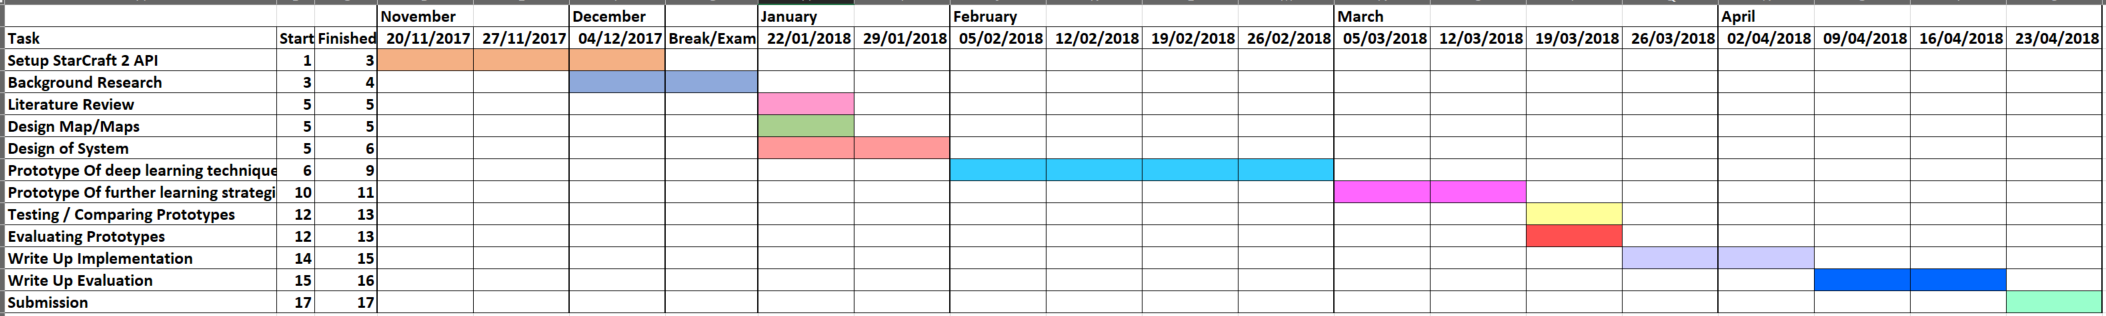
\includegraphics[width=1\textwidth]{gantt}
    \caption{Initial Time Frame}%
    \label{fig:gantt}
\end{figure}

It can be seen that the largest portion of time was given to the prototyping
stage. This was because the definitive scope of that stage is dependant on how
the project progresses, and which styles of learning end up being implemented and
being the most interesting. As such, whilst being a very long part of the project
on the chart, it will actually be made up of lots of small iterations, as described
earlier.

\subsection{Background Research/Literature Review}

In an Exploratory Software project, the research and literature review sections
are some of the most important, both in terms of understanding the problem
space the project is heading in, as well as understanding the styles of
solutions that have been used in both the area and other problems before.
This allows the problem to be fully understood, and to understand the work
and issues that come with various solutions. It can also help inform
the prototypes stage, by giving extra definition in how the prototyping stage
should progress, such as the styles of methods to test and the parameters to tune
in them.

\subsection{Prototypes}

After researching the problem and possible solutions, prototypes of various
solutions need to be produced. These prototypes can vary in both their approach
to the problem as well as being small iterative changes over a previous model
to tune certain parameters. A number of differing prototypes are useful for
various things, mainly to provide more conclusive evaluations later in the report,
since there will be more prototypes to compare against. It is also beneficial to
help identify what features of a prototype are the most useful, since networks
features can be compared and contrasted to see what features consistently give the
best behaviours.

The majority of the project is scheduled in this area, as there is a few
different techniques we can test, as well as further ones that will be found
during the research phase. Spending a lot of time to get a number of differing
agents increases the likelihood of finding what is needed to exhibit intelligent
behaviour and also increases understanding of the project space for further
prototypes.

\subsection{Modifications to Timeline}
%TODO: Fill this bit in. Explain why there were changes.

%TODO: Re-read this chapter since it was written before the project really got
%underway, and as such could have changed.

\chapter{Research}%
\label{research}

\section{Theory}

This chapter gives an overview of the existing research and methods that
have occurred in this area. This will first consist of a more descriptive
outline of the project space and the methods that can be used to tackle it,
before moving into talking about existing solutions and how they potentially
differ to the solution required in this case.

\subsection{StarCraft II}

StarCraft II (SCII) is a real-time strategy (RTS) game for PC released in 2010.
The game consists of many challenges that make it exciting for
teaching an automated agent to play. An example of the SCII in-game
interface can be seen in Figure~\ref{fig:scII}.

\begin{figure}
    \centering
    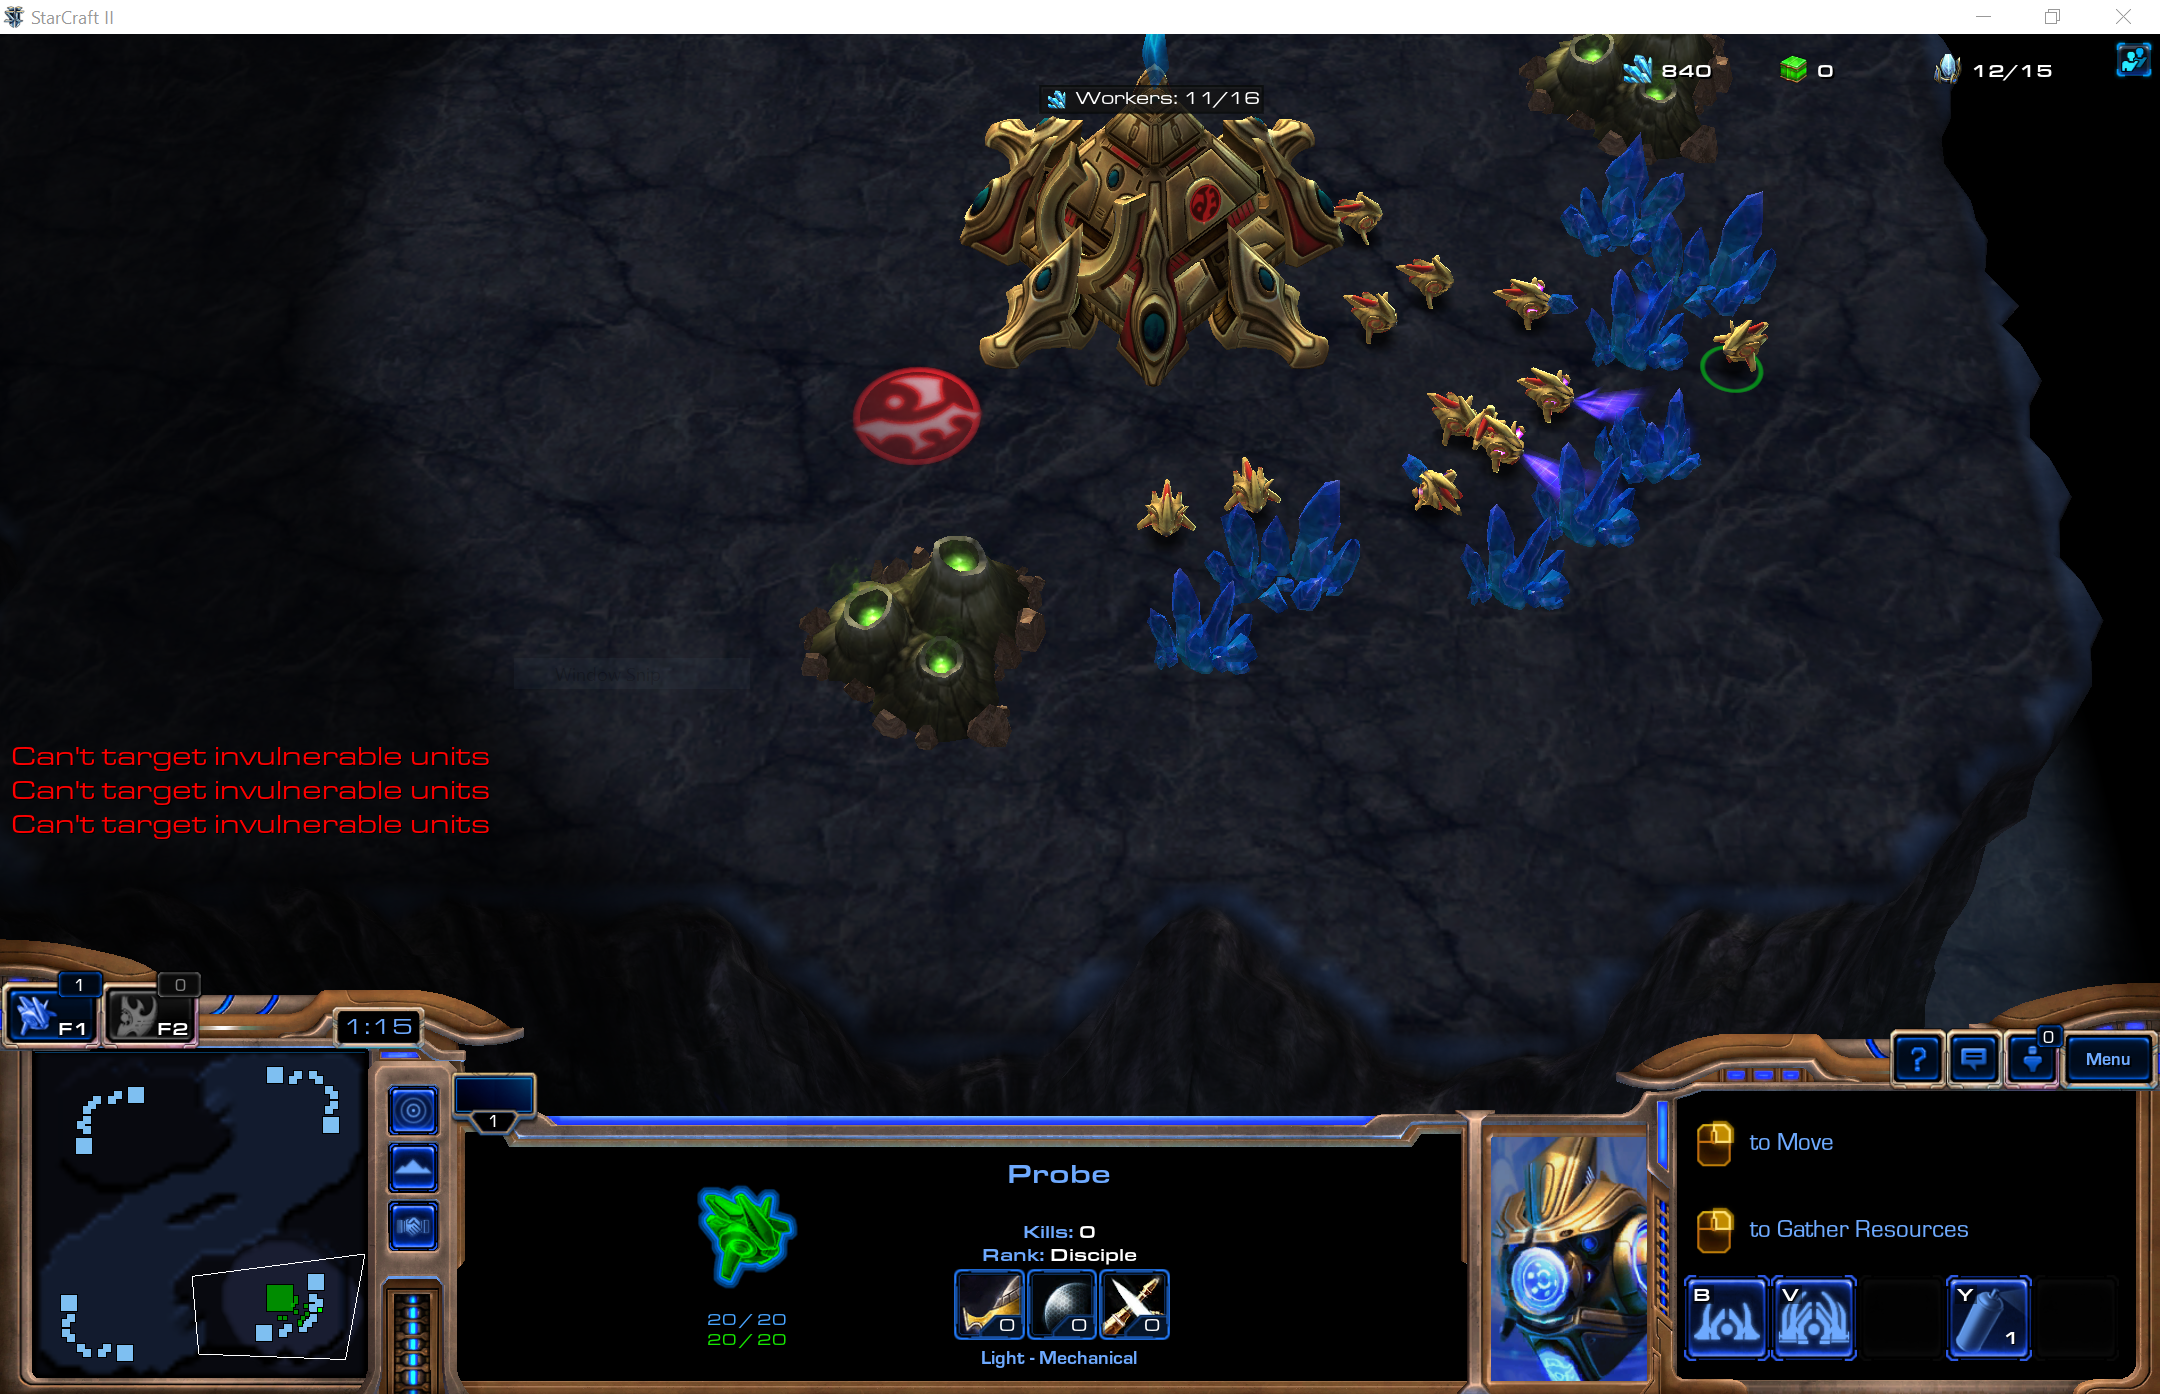
\includegraphics[width=1.0\textwidth]{scII}
    \caption{Example of the StarCraft II in-game interface.}%
    \label{fig:scII}
\end{figure}

A basic game of StarCraft II requires the management of the following:

\begin{itemize}
    \item \textbf{Resource Gathering}: Two types of resources must be gathered
        around the map, which in turn can be used to purchase additional units
        and buildings.
    \item \textbf{Unit Management}: StarCraft II consists of many
        units of varying types, which must all be given actions such that an
        efficient outcome is reached. For gathering units, this means having
        them always gathering resources of the required types or working on
        building the next required building, and for combat units
        this means controlling and utilising and their abilities effectively
        such that they are performing their best in fights. This also means
        managing the efficient spending of resources on new units.
    \item \textbf{Building Management}: Buildings must also be managed, which
        means building new buildings to either increase the maximum number of
        resources and units the player can have, or allow the building of new or
        additional number of units.
\end{itemize}

All of these actions take place on a large game map, where the player only has
partial information. That is, the player can only see the map where they have
units placed, anywhere else is shrouded in a so-called `Fog of War' which hides
any resources or enemy units which may be there. Because of this, the player
must scout the map to look for resources and the enemy, while also managing the
units and resources in their central base. In practice, this means a player is
expected to move the in-game camera back and forth around a large map, to send
and manage scouting or combat units, and jumping back to manage resource
gathering and base building at the central base.

All of these add up to many challenges for an intelligent agent to
overcome, as outlined in the next section.

Additionally, there is a significant competitive scene for StarCraft
II\cite{scIIprof}, which has a lot of potential benefits for training an
intelligent agent. It means there are many `Replays' from highly
skilled players, which could be used for supervised learning techniques, as well
as standards to compare against for unsupervised learning techniques.

\subsection{Issues with StarCraft II for an Intelligent Agent}

A game of StarCraft II includes many challenges for a player regarding
complexity. The game state can be comprised of thousands of different aspects
that could represent valuable information for the player. At a given moment,
there are potentially hundreds of different moves that a player could take,
which results in a vast action space. Plus, an average match of StarCraft II can
take between 10--15 minutes. Actions taken at the start of a game to build or
not build a potential unit type until later could result in the win or loss of a
game, meaning that every action needs to be thought out.

This means an intelligent agent for SCII would need to be able to evaluate all
these parameters too, and deal with the issues that come up in this style of
game, versus that of say Chess or Go. This will be spoken about in more detail
in Section~\ref{challenges:games}.

\subsection{Q-Learning Table}

Q-Learning is a reinforcement learning algorithm that uses a tabular approach to
state action pairs. Q-Learning is an off-policy method which gives the agent the
ability to randomly select actions in a given state without affecting the
updated value of the state action pair. Q-Learning requires:

\begin{itemize}
    \item State: some form of representation of the environment the agent is in.
    \item Action: an action that may move the agent from one state to the next
        or keep it in the same state.
\end{itemize}

The agent is given a state of the world and checks the lookup table for which
action would have the highest value in that state. The agent then executes that
action and rechecks the table again for the new state. Upon executing an action,
the agent may be given a reward, a value that dictates whether the action taken
was favourable or incorrect. The table can be updated through a real-time
learning or at the end of an episode. An episode represents an entire list of
states and actions taken to reach the end, usually by having a terminal state.
The table is updated using the Q-Learning equation. The algorithm is as follows:

\begin{itemize}
    \item The agent observes its current state
    \item The agent performs an action
    \item The agent observes the new state it is in
    \item It will also observe the new reward (if any are given)
    \item The table is adjusted for the previous state using a learning factor
\end{itemize}

The equation for updating the table is~\cite{watkins1992q}:

\begin{align}
    Q(s_t,a_t) = Q(s,a_t) + \alpha (r + \gamma (\max_a Q(s_{t+1}, a) - Q(s_t,a_t)))
\end{align}

The rewards are given as follows:

\begin{itemize}
    \item Immediate rewards: The agent is given a reward after an action is
        taken and the next state is not the final state.
        \begin{align} \label{eq:q_update}
            Q(s_t,a_t) = r + \gamma (\max_a Q(s_{t+1}, a))
        \end{align}
    \item Terminal rewards: The agent is given a reward and the state is the
        final state.
        \begin{align}
            Q(s_t,a_t) = r
        \end{align}
\end{itemize}

\subsection{Neural Networks}

Neural networks take inspiration from the biological neurons that
are present in the brain, similar to how genetic learning
algorithms take inspiration from the physical process of evolution
and mutation\cite{goldberg2006genetic}.

Broadly, a Neural Network is a model that estimates a function $f$.
It does this by using a set of weights, and input neurons. A neuron
can be thought of some model that given some inputs, gives
an output which is some weighted sum of the inputs.

A given network can have any number of neurons, connected in a number of
different ways. Typically, neurons are arranged into layers, which are sets of
neurons which are all receiving from a given input, be that an outside source,
or a different layer of neurons. An explanation of these layers will be given
later. The communication between the neurons is done by using the weights
mentioned earlier, where $w_{ij}$ denotes the weight between neurons $i$ and
$j$. Depending on the style of the network, there may be restrictions on the
values of these weights, and it is also possible that $w_{ij} \ne w_{ji}$.

For a value to be passed through the network, it is given as input to an input
layer, where it is then multiplied by the associated weights of the neuron the
value entered on, perhaps with the use of an associated activation function. A
common activation function is the Rectified Linear Unit
(RELU)\cite{Nair:2010:RLU:3104322.3104425}, which works by taking the maximum of
two values as follows:

\begin{align}
    f(x) = \max(0, x)
\end{align}

where $x$ is the input value to the activation function.

For an average network, the layout of the layers is an input layer,
followed by some hidden layers, and finally an output layer. Usually,
these layers are fully-connected, which means there every neuron in each
layer is connected to every neuron in the following layer, but
there are no connections between neurons of the layer. An example of this
is shown in Figure~\ref{fig:common_layout}.

\begin{figure}
    \centering
    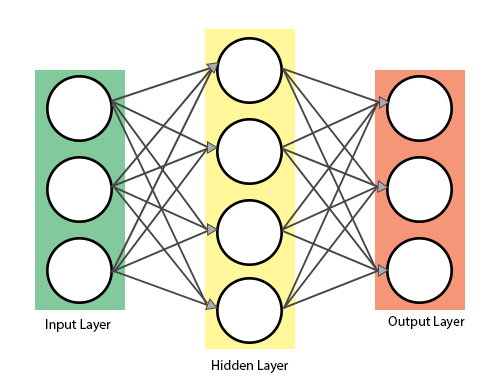
\includegraphics[width=0.6\textwidth]{common_layout}
    \caption{Common layout of a neural network.}%
    \label{fig:common_layout}
\end{figure}

\subsection{How a neural network `learns'}

For a neural network to function, it must go through a learning process, such
that it can sufficiently model the function it is needed for. This process is by
a set of functions $F$, where a solution $f' \in F$, and $f'$ solves the given
function best of all available solutions.

This leads to a need for a cost function, such that the best solution can be
found.  A cost function is defined as a mapping from the set of functions $F$ to
the real numbers, such as:

\begin{align}
    C : F \rightarrow \mathbb{R}
\end{align}

where there exists some optional solution $f^*$, which is bound as follows

\begin{align}
    C(f^*) \le C(f) \forall f \in F
\end{align}

which means that the cost of the optimal solution is bound by the cost of
all solutions in $F$.

With this, the process of the neural network learning turns into an optimisation
problem, that is, to choose the correct weights that sufficiently minimises the
cost function $C$.

The weights are picked randomly at first, before going through a tuning process
as the network is run. The specifics of this will depend on the style of network
and if a supervised or unsupervised learning method is being used, which will be
discussed later. Broadly, given these initial random weights, a training process
is used to tune the weights into being suitable. An input is received and
propagates through the network to the final output layer. Once an output is
given, it may be compared against some ground truth or metric, to evaluate if
the given output was suitable. If the output is suitable, then the next input
is received. However, if this is not the case then instead, the weights must be
adjusted, such that given the same inputs again, a more desirable result is
achieved.

Commonly, this is achieved via Backpropagation~\cite{hecht1992theory}.
Backpropagation is the process of calculating the required gradient, needed to
adjust the weights of the network~\cite{goodfellow2016deep}. However, this is
mainly used in supervised learning techniques, where a known value is available.

Backpropagation is achieved through repeated use of the chain rule, to go from
the output layer back to the start of the network, using the derived gradient to
update the weights in each layer, such that they are closer to a more optimal
solution. Essentially, this means calculating the error of the network for a
given value, and then propagating that error through the network from the output
back to the input, such that the weights move towards an optimal value, usually
with the usage of some learning rate value to prevent large changes in the
weights in a single step.

\subsection{Supervised and Unsupervised learning}

As mentioned previously, there is broadly two different styles of learning,
supervised and unsupervised learning (though there is some area between,
sometimes called semi-supervised~\cite{chapelle2009semi}).

The main differences between these two are how training is conducted. In a
supervised learning environment, there exists some dataset which has an
associated set of labels, such that learning can be done and any result can
instantly be checked against this ground truth, to help the process of
backpropagation. Unsupervised learning differs to this, where a known truth does
not exist, making the process of backpropagation much harder.

Commonly, the result of the outcome is instead used to help the
backpropagation process, but this can also be difficult. For example, in games
the result of an action may not be seen for hundreds or thousands of time-steps,
making the process much harder~\cite{sutton1984temporal}. This makes the
learning process harder since there is no ground truth that can be compared
against, instead, a metric that will change and adapt over a large period.

This can be avoided by using final results of a process, for example, using the
result of a game, rather than the score after some number of time-steps.
However, this has other issues, such as slowing the learning process and
potentially rewarding unproductive behaviour that occurred as part of a game
that eventually was won. The opposite is also true that actions that give a
local reward may still lead to failure to win the game. Because of this, it
makes the learning process more nuanced than merely comparing against a ground
truth. This can be experimented with to see how it affects learning.

\subsection{Deep Q Networks}

The main issue with using a tabular approach to keep track of state-action
values is the number of required entries. As a more complex space needs to be
represented, the number of entries in the table would increase for every
possible combination of values. The newest approach to tackling the issue of
complex space environments is to use a neural network. The weights represent
what an expected value for a given state could be. The state is given as input
into the network, and then the highest value output is chosen as an action to be
taken by the agent. Steps for running the network are as follows:

\begin{enumerate}
    \item A state is given as input into the network.
    \item The input is multiplied by the respective connected weights.
    \item The next layer is then given the input from the previous layer.
    \item The final output layer will return different values for each node in
        the layer.
    \item The node with the highest value represents the action to be taken.
    \item Once the action is taken, a reward value is recorded and used to
        update the network.
\end{enumerate}

The main difference between a Deep Q Network and a standard neural network is
the update function used. A Deep Q Network uses the loss function from the
Q-Learning algorithm to update the weights of the network. The loss function
provides a value of the target return and the predicted return. For example, the
agent could choose that in a particular state the best action would be the third
action with a value of 20. The agent takes the action and gets a returned reward
that is less. The network is then updated to return a lesser value for that
action next time the agent is in that state again. This is known as the TD
error:

\begin{align}
    TD Error = \sqrt{{(Q(s',a) - Q(s,a))}^{2}}
\end{align}

The error is the value difference between the next state reward and the
currently expected reward. This tells the network whether the expected reward
was correct or far. The value is then updated by increasing or decreasing based
on the returned reward~\cite{pandey2010reinforcement}.

The update could be applied in real-time or at the end of every episode.

When using a real-time learning environment, the agent is more likely to mistake
an action for being optimal from the first reward it gets. This makes the agent
tend to be more bias towards actions that get an immediate return and will not
allow the agent to see the possibilities of foreshadowing what could be a better
action in the long run. To avoid overfitting for a single environment, the agent
needs to be exposed to different maps and states. Updating the network at the
end of each episode may make the agent learn action pairs that are incorrect and
do not impact the reward factor. For example, the agent can move left, which we
may assume is correct, then go right and then left again. This introduces a loop
that the agent can get stuck in or an extra action step that is unnecessary.

To avoid such an outcome, a discount factor $\gamma$ is used to reduce the
reward value for an incoming state. So the more steps an agent may take to the
reward, the lesser the reward value is. Once the agent takes an action, based on
the state given to the network, the reward is observed and used to update the
Q-Target. The Q-Target looks at the next states and checks which action yields
the highest value return. That value is then used to update the current state in
the network by using the TD Error.

\begin{align}
    QTarget = r + \gamma*Q(s',a)
\end{align}

The prediction made by the network is then subtracted according to the TD Error
equation. This is then multiplied by the learning rate. Final update value
is:

\begin{align}
    Q(s,a) = Q(s,a) + \alpha (TDError)
\end{align}

The equation above is the same equation used in the Q-Learning algorithm.
However, it is implemented through the network with a gradient descent
optimiser. The network evaluates the loss function using the TD Error and then
updates the relevant weights. The learning rate $\alpha$ must be tested with
multiple values. If $\alpha$ is increased, then the network may converge to an
optimal value quicker but may also tend to overshoot the local minimum and
diverge from the optimal value. This makes $\alpha$ a critical hyper-parameter
based on the amount of training the agent may have. If the $\alpha$ value is set
to a lower value, then the agent will require more training to achieve an
accurate estimate of the expected reward for a given state action pair.

\subsection{Convolutional Neural Networks}

A Convolutional Neural Network (CNN) is a type of Artificial Neural Network
(ANN). Broadly, a CNN is similar to that of an ANN, in that it consists of some
neurons that have associated weights and receive some input, be that from an
input layer or another layer of neurons. Where they differ though is that with a
CNN it is assumed that the input is an image, which changes the learning
procedure and design principles.

To give an example of why this style of network is needed, the size of a non-CNN
network must be considered. For the MNIST~\cite{lecun2010mnist} dataset, the
supplied images are $28 \times 28$. For a fully connected architecture, this
leads to $28 * 28 = 784$ weights. If an RGB image is used, this number is
multiplied by 3 to get the number of pixels in each of the three channels. $784
* 3$ weights is reasonable, but once moving to an image of a more reasonable
size, say $(250, 250, 3)$, the number of weights becomes very large, without
even considering the rest of the neurons in the network.

A CNN works differently, however. Since it can assume the input is an image, the
network architecture may be built in a more specific way. That is, instead of
input consisting on a flat vector of numbers, the input may be considered in 3D,
where the images vertical and horizontal resolution make up the width and height
of the input and the depth is made up of the channels the image is made up of,
traditionally 3. This is then helped further as the neurons in this 3D layer are
only connected to a small receptive field from the input image, rather than the
entire input like in a fully-connected network. Broadly, it can be said that a
convolutional layer takes a 3D input and transforms it to some 3D output. In the
context of the MNIST dataset, this would be the classification. An example of
this 3D network can be seen in Figure~\ref{fig:cnn}. It can be seen that the
image is given and is transformed into a second 3D volume of the same size, but
with additional channels.

The additional channels once the convolutional layer has been processed is due
to the number of filters in that layer. These are defined as the area the neuron
in a given layer connects to on the input. For example, a neuron in the first
layer may look at a $3 \times 3$ section of the input, extending across all
channels of the input. This filter is applied to the entire image by moving it
over every pixel combination it fits on, and at each location, the dot product
on the input and the values in the filter is computed. For the whole image $I$
and a filter $F$, this is defined as follows:

\begin{align}
    {(I*F)}_{xy} = \sum^{h}_{i=1} \sum^{w}_{j=1} F_{ij} \cdot I_{x+i-1, y+j-1}
\end{align}

which means that for a given a $(x,y)$ position, the value of the filter at that
point for a given filter is the dot product of each value in the input and the
value in the filter.

These filters are stacked, which then increases the receptive field of the later
layers. This process was mirrored on features found in
biology~\cite{hubel1968receptive}. The receptive field refers to the area that a
given neuron is receiving input from. For the first layer, this is merely the
size of the filter, for example the $3 \times 3$ grid. However, this layer is
then used as input for the next layer. It can be said that the second layer's
receptive field relative to the image for a filter of size $3 \times 3$ is
5. This increases throughout the network, building up evermore complex and
abstracted representations of the image, that are increasingly global across the
image. This can be seen in the filters that are calculated in the network,
where the earlier layers contain low-level features, where the later
ones become more abstract and cover more significant parts of the image,
as shown in Figure~\ref{fig:filter_example}.

In general, the formula a given layer $l_k$, the receptive field can be
calculated as follows:

\begin{align}
    l_k = l_{k-1} + ((f_k - 1) * \prod_{i=1}^{k-1}s_i)
\end{align}

where $f_k$ is the filter size of layer $k$ and $s_i$ is the stride for the
$i^{th}$ layer.

\begin{figure}
    \centering
    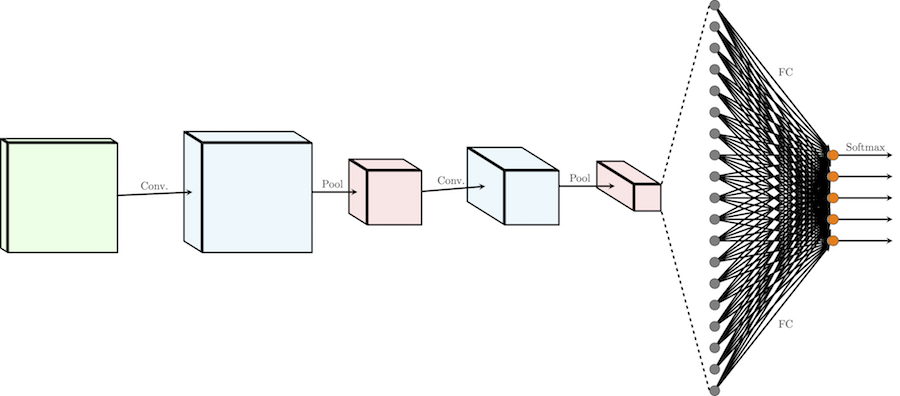
\includegraphics[width=0.9\textwidth]{cnn}
    \caption{Common layout of a convolutional neural network, from
    Cambridge Spark\cite{cnn-layout}.}%
    \label{fig:cnn}
\end{figure}

\begin{figure}
    \centering
    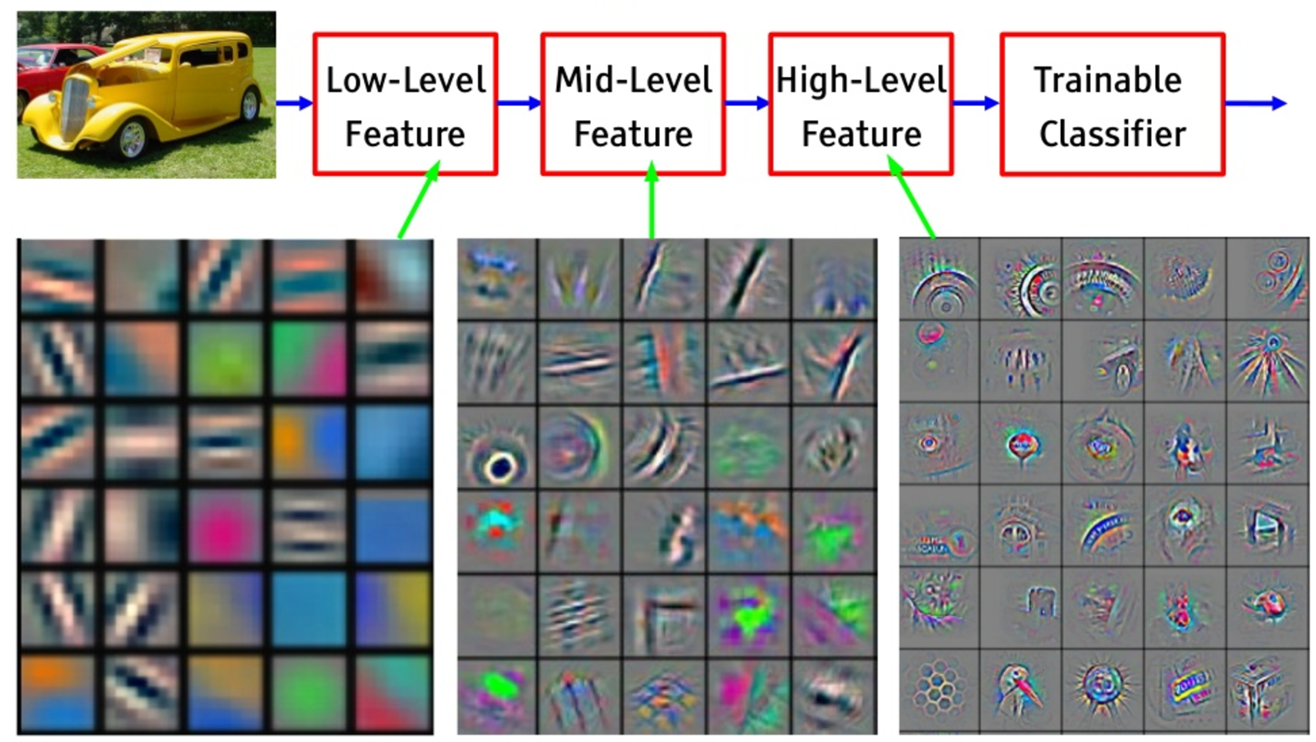
\includegraphics[width=0.9\textwidth]{filter_example}
    \caption{Examples of filters from various layers, from
    NIPS'2015 Tutorial\cite{filterexample}.}%
    \label{fig:filter_example}
\end{figure}

\subsubsection{Other required techniques}

There are other techniques that go alongside a CNN by default and have been
mentioned previously. This includes both pooling layers and the concept of
striding which is used both in the pooling layer and also the convolutional
layer.

When a filter uses a stride, the filter is moved by more than a single pixel
each time. By default, a stride is 1, that is it is applied to every single pixel
on the input. However, it is also common to have a stride of two, or in some
rare cases, a stride of greater than 2. When this is the case, the filter
is moved two pixels at a time, rather than 1. This leads to less overlap in the
receptive fields but does have the potential downside of reducing the
resolution of the input.

A pooling layer is a form of down-sampling. Given an input, the pooling layer
will reduce the resolution of it in some fashion. The most common pooling layer
used is the max-pooling layer. This layer takes the maximum value in a filter
and uses that as the value for that filter. This is commonly done with a filter
of size $2 \times 2$ and a stride of 2. The result is an image that is halved
in both the width and height dimension. This is useful to help reduce the number
of parameters in a given network, so is commonly applied after each
convolutional layer. An example of a max-pooling layer can be seen in
Figure~\ref{fig:max_pool}.

\begin{figure}
    \centering
    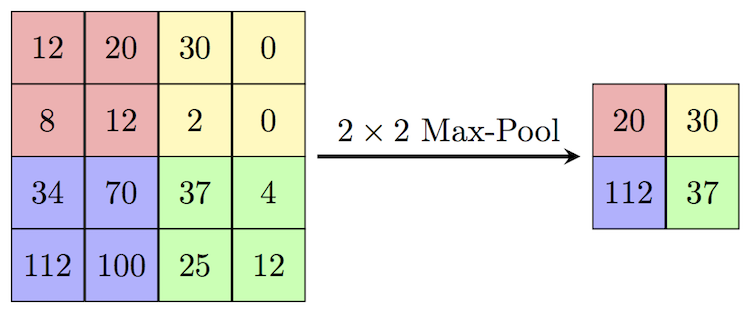
\includegraphics[width=0.9\textwidth]{max_pool}
    \caption{Example of max-pooling, from Computer Science Wiki\cite{max_pool}.}%
    \label{fig:max_pool}
\end{figure}

\subsection{Transfer Learning}

Transfer learning is a process in machine learning that describes the practice
of use knowledge learnt from one problem to help solve a different problem. The
second problem needs to be a different but related problem for transfer learning
to be useful. A typical example that is used to describe this process is that a
network that has been trained to find cars in an image could be used as the
basis of a network to locate pictures of trucks, vans or other vehicles.

Transfer learning can be useful for many reasons, the most obvious of which is
lowering the complexity of the new task, due to the network having existing
knowledge. This works best when the task at hand has not significantly changed,
but the domain has. A good example of this is the use of transfer learning in
medical applications, where knowledge in one domain can be very quickly applied
to another\cite{van2015transfer}. However, what is perhaps less obvious but more
useful, is the ability to augment an existing small dataset by using a network
trained on another domain entirely, for example using networks trained on the
ImageNet dataset\cite{ILSVRC15}, for use in entirely different domains such as
medical imaging\cite{shin2016deep, tajbakhsh2016convolutional}. This is possible
due to the task at hand, recognising some feature or object, has stayed the same
despite the vast differences in the domain.

A more formal definition of Transfer learning follows, as taken from ``A
Survey on Transfer Learning''\cite{pan2010survey}.

Given a domain $\mathcal{D}$ this is made of a feature space $\mathcal{X}$, and a
probability distribution of $P(X)$ over $\mathcal{X}$, where $X = x_1, \ldots,
x_n \in \mathcal{X}$.

A task $\mathcal{T}$ for a domain $\mathcal{D} = {\mathcal{X}, P(X)}$ consists
of $\mathcal{Y}$, a label space for the task at hand, as well as $P(Y|X)$ which
is the probability of a label $Y$ from some training data $X$, typically for
some pair $x_i \in X$ an $y_i \in \mathcal{Y}$. These labels are specific to the
domain in question, so for the MNIST dataset, they would be the numbers zero
through nine.

Finally, transfer learning can be defined as given a source domain
$\mathcal{D}_s$ with an associated task $\mathcal{T}_s$, alongside a target
domain and task $\mathcal{D}_t$ and $\mathcal{T}_t$, transfer learning aims to
learn the task of the target domain, using information from the source domain.
This is expressed as wanting to learn $P(Y_t | X_t)$ in $\mathcal{D}_t$ using
information from both $\mathcal{D}_s$ and $\mathcal{T}_s$, where either
$\mathcal{D}_s \ne \mathcal{D}_t$ or $\mathcal{T}_s \ne \mathcal{T}_t$.

This definition of the problem leads to four scenarios of transfer learning,
where each of the four elements that make up the $\mathcal{D}$ and $\mathcal{T}$
tuples are different.

\subsection{Curriculum Learning}

Curriculum learning is a similar process to that of transfer learning. However,
where it differs is that in transfer learning, knowledge learnt in any domain or
task is used to make a similar task easier. In curriculum learning, it is
instead the idea that learning information in a specific order can improve the
speed of convergence to some local minima, and in some cases improve the local
minima found.

This idea takes its inspiration from the fact that humans learn this way. Humans
are rarely given information in a random order; instead, they are given it in a
specific order of increasing difficulty to progress through. This can be applied
to machine learning by curating the order examples are passed to a network. This
can be as simple as preparing for training with a single small set of easy
examples, or as complicated as a full sequence of increasingly tricky cases.

Formally, this process can be defined as followed, as using the equations
outlined in ``Curriculum Learning''\cite{bengio2009curriculum}.

Given $z$, a random example for the network (or $(x, y)$ for a supervised
example and its associated label), let $P(z)$ be the target probability
distribution that would learn the required function. Let $0 \le W_{\lambda}(z)
\le 1$ be the weight applied to $z$ at step $\lambda$ in the curriculum, with
$1 \le \lambda \le 1$ and $W_1(z) = 1$. That leads to the following training
distribution at a step $\lambda$:

\begin{align}
    Q_{\lambda}(z) \propto W_{\lambda}(z) P(z) \qquad \forall z
\end{align}

such that $\int Q_{\lambda}(z) dz = 1$. This leads to

\begin{align}
    Q_1 (z) = P(z) \qquad \forall z
\end{align}

This allows us to consider an increasing sequence for $\lambda$ such that it
increases from 0 and ends at $\lambda = 1$.

This allows curriculum learning to defined as a sequence of distributions of
$Q_{\lambda}$, which we may call a curriculum if the entropy of the
distributions increases:

\begin{align}
    H(Q_{\lambda}) < H(Q_{\lambda + \epsilon}) \qquad \forall \epsilon > 0
\end{align}

and $W_{\lambda}(z)$ (the weights) are monotonically increasing (that is, always
increasing) in $\lambda$:

\begin{align}
    W_{\lambda + \epsilon}(z) \ge W_{\lambda}(z) \qquad
    \forall z, \forall \epsilon > 0
\end{align}

Broadly, this means that as we increase $\lambda$, that is by adding new
examples, $Q_{\lambda}$ also increases alongside $\lambda$, as the training
examples move from a set of small, easy examples and finishes with the full
training set. As $Q_{\lambda}$ is increasing and is proportional to the weights
and the probability distribution, the network is converging towards a better
minima.

The exact definition of what consists of an `easy example' will depend on the
domain, and can be experimented with as part of the final model's evaluation.

\section{Challenges}

Reinforcement learning has many challenges, both specific to this
project, and those that are issues for reinforcement learning as a whole.
This section aims to outline these challenges, as well as ways they have been
mitigated in other projects and how these fixes may apply to this project.

\subsection{Reinforcement Learning For Games}\label{challenges:games}

Reinforcement learning for games is particularly tricky, which is what makes it
an exciting research area. Games provide a suitable test-bed for some broader
issues in the area, while also providing a repeatable environment for running
tests.

There has been recent success playing older games using reinforcement learning,
such as games on the Atari 2600\cite{mnih2013playing} and
Doom\cite{kempka2016vizdoom}.

Both of these examples had to overcome the following issues:

\begin{itemize}
    \item `Labels': For traditional deep learning applications, a large dataset
        with associated labels is needed. However, in this case, we instead must
        learn from a reward, which is usually delayed for a number steps. For
        example, a reward may not be given until the game is finished, in which
        case it is tough to link early actions to the reward. The first
        action taken could have a strong correlation or no effect on the final
        score, but tracking it over an entire game can prove very difficult.
    \item Independence of Inputs: Most deep learning algorithms assume that
        all inputs are independent, which is usually not the case for
        reinforcement learning. This is usually because in reinforcement
        learning each state follows the last, in this case as frames of input
        from the game. This can cause issues due to the network needing to
        understand that a given state leads to another and so on.
    \item Action Space: In games, there is usually a vast number of actions that
        a player can take at any given moment. This can be in the form of either
        the number of actions or the number of locations a given action can
        take place at. Shooting at one spot is not the same as shooting at
        another. This usually means that both an action and location pair is
        required.
    \item Incomplete Information: Unlike in most forms of supervised learning,
        reinforcement learning commonly has elements of incomplete information,
        that is there is missing information. This is not always the case, such
        as in Go or Chess, but most games have elements of missing information.
        This makes it more difficult to decide since the full state is
        not available.
\end{itemize}

However, there are also things which are much easier to use in reinforcement
learning, such as learning with self-play that is having an agent play against
another agent. This has been used in Poker\cite{heinrich2016deep}, Chess and
Shogi\cite{silver2017mastering} and most recently
Go\cite{silver2016mastering,silver2017masteringgo} to great success.


\subsection{StarCraft II specific issues}%
\label{sc2-issues}%

StarCraft II specifically offers an environment that offers a lot of interesting
challenges.

First, there is the issue of associating a reward with an action. This is
especially an issue for StarCraft II for a few reasons. The main of which is
the rate at which actions are taken is incredibly high, especially in high-level
play. Professional players can hit upwards of 150 actions-per-minute
(APM)\footnote{Value is taken from:
\url{http://starcraft.wikia.com/wiki/Actions_per_minute}}, which over an average
game of 10--15 minutes, combines to numerous actions that need to be given and
later have a given reward associated with them. This can be avoided if a supervised
learning approach is taken. As mentioned previously, there are many `game
replays' available, from all styles of games. These replays contain the full
game and all actions taken, so can be used to either augment a reinforcement
learning approach, either through starting a network or helping an existing
network learn. This approach has been used to varying success in similar domains
such as Atari games\cite{hester2018deep} and also the original StarCraft
game\cite{justesen2017learning}.

Replays also help the second issue, which is incomplete information.
A game of StarCraft II takes place on a potentially large map, with up to 8
players simultaneously playing on the standard maps. This means that an agent
could be missing out on the information of 7 other players. Both the number of
players and the size of the maps lead to a significant amount of missing information.
However, replays do not have this restriction, and as such both players and bots
alike can use replays to analyse both their own and other players strategies to
improve their play.

Similarly, due to the large map and the wide range of units in the game, there
is a significantly large action space at any given time. Compared to a game like
Chess, where there is a (comparatively) small number of units, actions and
spaces to perform those actions, SCII has an order of magnitude more actions
available, meaning an agent has more options they must perform. Similarly, there
are many moves that require complex planning, such as `Build a
combat unit', which may take many steps to reach, such as gather
resources to some amount, build a building to build that specific unit, wait for
the building to be complete, and finally, queue the building of the required
unit. This sequence of actions and more complicated ones need to be learnt to
be a successful SCII player.

Additionally, compared to a game such as chess or even the Atari games,
StarCraft II consists of multiple in-game characters which must be controlled.
In Chess, a single piece is moved each turn normally, whereas in StarCraft II a
group of units must be moved, which means selecting the required units and
moving them. This complicates the movement action as it is now depends on a
selection step. This is made more complicated due to the limitations of the API
making selecting certain units from a group much harder.

\section{Existing Methods}

There are many existing methods in the area of reinforcement learning for games,
as well as solutions that fall outside of gaming but are still potentially
relevant.

For example, there is existing research into applications for the original
StarCraft game, where some different methods were tested. The methods vary
wildly, and a few examples are given now.

The paper ``Reinforcement learning agents providing advice in complex video
games''~\cite{taylor2014reinforcement} talks about using a system to train a
network, given guidance from a teacher. It discusses the use of having a network
be a `student' such that it takes instructions from the teacher as it learns to
guide its learning, though this process can only be used a certain number of
times. The conclusion reached shows that given suitable advice, an agent can
learn much faster. While interesting, this style of learning is not readily
compatible with the use of curriculum or transfer learning, which limits its
usefulness in this project. However, it could be an exciting extension in the
future.

There are many papers on the use of reinforcement learning for the original
StarCraft game and its expansions~\cite{wender2012applying,
shantia2011connectionist}. However, many of these solutions had issues with the
processing of the system, such that they had to develop novel systems to even
get the data out efficiently, which is not a problem with the SC2LE\@. Despite
these issues, they managed to get intelligent behaviour out of the respective
agents either in full games or in small problems that were subsets of the full
game. Both of these agents used a Q-Learning approach or a Sarsa learning
approach~\cite{sutton1996generalization} to differing results. The results
achieved as well as the methods used could prove useful informing design
decisions for the networks used for this problem. However, due to the change in
both the game and the method that is used to interact with the game, the
techniques and parameters used could prove to be less useful due to a
significant difference in the two environments.

Finally, the last area that can be used for inspiration is the vast amount of
work that has been done in the field of reinforcement learning throughout gaming,
rather than the work that is specific to StarCraft. While older games such as
the Atari 2600 games mentioned above, differ massively from StarCraft, there are
more modern games that have similar problems. For example, the game
Civilization IV~\cite{wender2008using}, which is a complicated strategy game,
taking place over a map that covers a large number of playable spaces, with
games taking many thousands or millions of steps potentially, depending on the
game settings. As such, similarly to StarCraft, the game has significant issues
with associating rewards and choosing the location that actions should be taken
at. As a result, most research is done on small subsets of the game. This
strategy again uses Q-Learning and could provide useful insights into the
design for a network for StarCraft II\@.

\section{Formal Definition of the Problem}

The final part of the research was into the problem of creating an intelligent
agent for StarCraft II\@. The previous sections cover all the technical aspects
that would be needed for such an agent, but does not attempt to define what
consists of an intelligent agent, nor what is required to consider the project a
success.

As mentioned, the game of StarCraft II consists of many elements, such that the
scope of an intelligent agent must be restricted, for it to remain feasible.
Because of this, the game will focus on two specific tasks: The DeepMind
mini-games and the Simple64 map. Both of these are explained in more detail in
Chapter~\ref{implem}.

Intelligent behaviour is hard to define, due to the inherent subjectivity in
determining what it consists of. This is spoken about in more detail as part of the
Evaluation Methodology in Chapter~\ref{eval_method}, but broadly the definition
used for this project is that intelligent behaviour is taking the most direct
route to a given solution or state possible, without having too many superfluous
actions. This means an agent does not necessarily need to reach a most optimum
state, as it is also true that many humans play games sub-optimally. However,
the agent should still efficiently move to that state.

To give a more structured example, consider a single agent has to move to
a set location. It may be quickest to follow a specific path, but the agent's
behaviour will be regarded as intelligent if it can move directly to the
target location, without unneeded actions such as turning around or attacking at
random on that path. The agent does not necessarily need to follow the optimal
path, but for such a simple example it could be expected that it would. This
expectation, however, would change depending on the complexity of the task.

\subsection{Solution Choices}

From the research that went into this chapter and the associated similar
problems, two styles of a solution will be built and tested.

First, a Q-Learning approach will be taken. This approach has been tested across
many different games and should prove very useful for this task. If combined
with compound actions that combine multiple actions into one single agent
action, it is possible that an agent may be able to show intelligent behaviour
across the many different test situations, to give a strong result. This
approach has the advantage of being used very readily across a vast number of
projects, including StarCraft and StarCraft II projects, as well as many other
games.

Secondly, a Convolutional Neural Network approach will be taken. This approach
has less testing, but a form of CNN did behave the best in the DeepMind SC2LE
paper~\cite{vinyals2017starcraft}, so there is proven results in the area that
show a CNN performs very well at this task. This approach should be more global
since it takes input of the entire visual space, and perhaps other additional
information, to learn its environment sufficiently.  However, it is also
possible that due to the higher complexity of being forced to select more
specific actions instead of the Q-learning approaches compound actions, it may
fair worse for tasks that require large amounts of tasks that take multiple
steps.

Both of these networks will allow research into Transfer and Curriculum
learning, such that their effect on both the learning speed as well as the agent
efficiency can be measured and compared.

Using the insights the many past projects gained should mean that a solution
can be found that avoids the issues outlined in~\ref{sc2-issues}. This mix of
solutions should also give an interesting comparison between the different
learning styles, and how each one fair for a given challenge.

\section{Conclusion}

In conclusion, this chapter has formally defined the required theory behind
neural networks, as well as both Deep Q networks and Convolutional Neural
Networks. Following this was an evaluation of the challenges the project could
face as well as the methods that have been attempted in and around the area,
such that they also may be considered here. Finally, a formal definition of the
problem and the solution choices based on the research gathered was given.

The network styles were chosen due to their proven results in the area, across
multiple games and project styles. These existing projects and deeper
understanding of the project area should give the created solutions more depth
and allow more informed decisions to be taken, as well as avoiding pitfalls that
may have been met otherwise.

Following this research, preliminary designs for networks can be made, to allow
the testing of the methods outlined here, as well as the later evaluation of
their performance, with a better idea of what constitutes an intelligent agent.
The following chapter will go into details of the design choices that went into
the design of the final networks, before outlining the performance metrics and
the achieved results.

\chapter{Implementation \& Design}
\label{implem}
\section{Environment setup}
Since the game is very complex and can consist of many possible action spaces, the majority of the experimentation focuses on the \textbf{Simle64} map. The map contains a single opponent and 2 starting bases. The agent is spawned into one of the 2 areas randomly and starts out with the \textbf{SCV} units, characters for building and mining. The initial stage begins with mining of necessary of resources for progressing through level by creating the required buildings and training \textbf{Marines}, fighter characters. This requires the agent to control the \textbf{SCV} and \textbf{Marine} units using complex three action commands.

\section{Q-Learning Table}


\section{Deep Q Networks}


\section{Convolutional Neural Networks}
\chapter{Evaluation Methodology}%
\label{eval_method}

\section{Datasets}

The two agent types will be tested on two different sets of datasets.
These are the DeepMind mini-games, as well as the Simple64 map. These two
datasets should give an overall idea of how the agent is performing.

\subsection{Mini-games}

The mini-games consist of small, constrained challenges that represent
small parts of the full game of StarCraft II, allowing simple actions
in the game to be tested, as well as compared against a range of
published scores.

Every mini-game has a time limit, and the objective is to get the
highest score possible in the time frame. The scores for the game are surfaced
as part of the SC2LE \texttt{obs} object, meaning the agent is capable of easily
telling how well it is doing, and learning from this reward.

These mini-games are:

\begin{itemize}
    \item MoveToBeacon: A simple map with a single marine (player controlled
        unit) and a beacon, which acts as a target to move to. The agent gets
        a point each time it reaches the beacon, at which point the beacon's
        location is reset.
    \item CollectMineralShards: A map with two marines and 20 mineral shards,
        which act as items to pick up. Once all are picked up, 20 more are
        placed on the map. To achieve an optimum score, the two marines must
        be controlled independently, which results in this map being
        harder than the MoveToBeacon map.
    \item FindAndDefeatZerglings: A map with three marines and 25 zerglings,
        which are an enemy unit. A point is achieved for each zergling that
        is defeated, and a point lost any time a marine dies. This map
        is also the first to deal with the moving of the camera, as the previous
        two games had the entire state visible without moving the camera.
        Upon defeating the 25 zerglings, 25 more are added.
    \item DefeatRoaches: A map with nine marines and four roaches, which are a
        different enemy unit. This requires a more complex strategy to defeat,
        and also on defeating all four roaches, four more are spawned as well as 5
        more marines. This means the number of marines potentially grows
        throughout the game. However, a point is lost for any lost marines.
    \item DefeatZerglingsAndBanelings: A map with nine marines and six zerglings
        and four banelings. This again needs a different strategy and also gives
        extra marines upon defeating all the enemies.
    \item CollectMineralsAndGas: This map requires more strategy than the last.
        The map starts with 12 SCVs (which are gatherer units), a command centre
        (which is used to create additional units) and two types of collectable
        resources. The objective is to gather as many resources as possible, and
        also intelligently build more gathering units to increase the
        speed at which resources are gathered. An optimal strategy will also
        build an additional command centre.
    \item BuildMarines: This is the last and most complex map. The map starts
        with 12 SCVs, a command centre and eight resources to collect. The
        objective is to build as many marines as possible in the time limit.
        This requires the building of Supply Depots to store resources and
        barracks to build marines.
\end{itemize}

All of these mini-games have published scores for the many different
techniques as well as some baseline scores for human players and random
policies. This makes them ideal for testing a model again, such that the scores can
be directly compared.

\subsection{The \textbf{Simple64} Map}

The \textbf{Simple64} map was also chosen to allow experimentation on a
straightforward version of the full game, where the challenge is to beat the
games AI, which is built using more traditional game AI technology, and also can
cheat at higher difficulties.

The map contains a single opponent and two starting bases. The agent is spawned
into one of the two areas randomly and starts out with the \textbf{SCV} units,
characters for building and mining. The initial stage begins with mining of
necessary of resources for progressing through the level by creating the
required buildings and training \textbf{Marines}, fighter characters. This needs
the agent to control the \textbf{SCV} and \textbf{Marine} units using complex
three action commands. The end goal is to defeat the AI player and win the game.

One aspect that makes this much harder is the removal of a simple scoring
element, like that in the mini-games. This means the only scoring methods
available is the win/lose/draw score at the end of the game, of the ``Blizzard''
score that is given throughout, but is based on many different in-game aspects.
This makes it much harder for the agent to directly tell how well it is doing in
the global aspect of the game.

The more obvious element that makes this harder is that it combines all the
tasks that the mini-games cover, as well adding new tasks as the AI player will
attack bases and units, search and take resources, and build units and
buildings, all of which are not covered in the mini-games. This combination of
both new elements and a large number of already known elements makes the simple
64 maps much harder to play.

Due to this map containing a small snippet of the entire game, it will be useful
for measuring how the agent behaves in a general settings, as it is possible for
an agent to excel at each of the underlying tasks that go into a game of
StarCraft II, but to fail in the process of combining them effectively.

\section{Reasoning For Evaluation}

Evaluating the networks is essential for many reasons. Firstly, with the
mini-games the networks can be directly compared to both each other and also the
list of existing results, which is very useful for giving a direct metric for
the agents. Secondly, the Simple64 map is useful since it allows a lot of
interesting evaluations, both in the measuring of how the agent has generalised
from the individual tasks but also for how the agent does in a full game of
StarCraft II\@.

The accuracy of the agents is vital so that we can see if the agents have
started to learn the basics of the game. This is particularly easy as we can
rank how they perform against published results, to see if they rank higher than
random or straightforward agents, as well as comparing against the human
player's scores that are given. It is expected that both agents will perform
well and similar to each other for the first few mini-games before the more
complex ones should split them up further and show their inherent advantages and
disadvantages in their implementations. These compromises can then be compared,
to see which agent performs the best, and also to see what features of each
agent is the most desirable if a newer agent was to be built using the
information learnt from this project.

Generalisation is similarly crucial in that it allows us to see if an agent that
has learnt the basics of the game can then apply the lessons it has learnt to
situations that use the same skills but take place on a different map. This is
important for the agent, as it should be able to apply its skills regardless of
the map, like that of a human player. Furthermore, this is useful for giving
additional information on how the agent has learnt in the initial case. It is
possible the agent was able to learn some feature of the map at hand that
allowed it to do well in a mini-game, but when applied to a more realistic case,
the agent fails. Testing across new areas should allow this to be caught, as
well as giving an insight into how the agent would potentially fair if put on an
arbitrary map.

\section{Measuring Accuracy}

Identifying the accurate action to take in an ever increasing space of
possibilities can be difficult. The main definition of saying how accurate an
agent is in taking an action will mostly depend on the final score achieved
through that episode. The game is being played in real-time and as so creates
complexity in the number of possible state action pairs that can be observed.
When the agent is playing in real-time, without any form of turn based playing,
the state space is too large to efficiently represent using a tree structure of
all possible actions.

This means that when measuring the accuracy of an action, it will depend
on the final score. For example, the agent can go up or down and then go to the
right and attack an opponent on the square in-between. To achieve the same
reward for both actions, would mean that the optimal action to take could be
either.

The main items that an agent must able to do is learn and improve. The learning
phase can be tested and shown by accumulating the loss function's value. These
values can then be analysed for a decline in values as more episodes are tested.
The loss function shows how far the policy's prediction was for a given action
and reward. As the agent trains, the predicted value and actual value should
converge. However, due to the random initialization of each episode in a
mini-game, the process of identifying the correct sequence and pattern is
difficult since the agent will keep learning the wrong pattern. Because of this,
the loss function will never perfectly converge to zero. This also keeps the
agent from over-fitting a single sequence of actions to take.

The final score of each episode is used to identify if the agent is learning the
correct actions to take. The agent should aim to maximize this value at all
times. When graphing the final score of multiple episodes, an increasing slope
will define the agents performance with the training it had already done. If the
agent is learning and improving the policy, then the average of final scores
should increase.

\section{Measuring Generalisation}

Since the agent is being trained on a curriculum based system, the required
movements and actions the agent needs to take will be learnt on different
mini-games that focus on different skills. The agent will be trained on
different mini-games using the same model. So if a mini-game is focused on
moving to the beacon, the agent will learn the required state and action pairs
for achieving the highest score possible on that map. This allows the agent to
train on specific scenarios with a specified outcome. Ideally, training on one
of these scenarios should not affect the other actions that are not required.
But there may be some overlap with the neural networks weights being affected
from each given action. An agent could be learning on a mini-game that requires
it to attack. This would then reduce the weights of other non-attacking actions
such as building or moving.

In order to measure the agents ability to generalize a given skill, the value of
a given policy will not work due to the issue of the agent reducing the value
policy of other actions. Instead the agents skill should be applicable to the
relevant field and tested on similar mechanics. So, an agent cannot be trained
on attacking and then tested on building. The agent should be tested on the same
actions but in different maps and scenarios.

%TODO: This subsection is great for generalisation, just needs a little extra on
%subjectivity of the actions. The definitive scoring of the mini-games means if
%they mess around, the scores will be lower. Here, they could wander around the
%map and still potentially win. So talk about that etc.

\chapter{Performance Evaluation}%
\label{eval}

This chapter, the performance of both of the networks outlined in
Chapter~\ref{implem} will be evaluated, such that their performance at playing
the game StarCraft II can be measured. The exact methodology for these tests is
described in Chapter~\ref{eval_method}.

Each section will be split into three, first evaluating the Deep Q network,
second the Convolutional network, and then finally comparing the two. The
results will mainly focus around the score achieved, which is the in-game is the
final score for the mini-game at hand, and for the Simple64 map, this will
compare how the bot fairs across 100 games against various bots. For the
mini-games, the overall comparison will allow comparisons with known baselines,
such that we can show how the agents stack up. For the Simple64 game where this
is not possible, it will instead focus on how the agent plays.

After this has been done for both the mini-games and the Simple64 map, the
results will be compared overall to see what the advantages and disadvantages of
each network is, as well as comparing other parts of the networks such as
training time, and robustness.

Finally, before the conclusion, some of the additional parts of the trained
networks which are not directly linked to the performance of the network, but
do give insight into how the networks works will be shown. For example, the
filters for the Convolutional network will be given here, as well as some
example outputs.

\section{Mini-games}

The mini-games are specific maps designed for training and testing different
skill requirements from the player. Each mini-game uses a different scoring
system, map and end goal. This makes it ideal for testing the agent on different
abilities for the agent to learn. Most of the mini-games incorporate some form
of randomness so that the agents do not learn to play using the same fixed
move-set. Because of this, the mini-games will be played 200 times with a
trained agent, and the mean and max scores will be recorded. This will allow a
suitable average to be taken, which takes into account the inherent randomness
of the mini-games.

For comparison, the results achieved by DeepMind are given in
Table~\ref{tab:deepmind}, as taken from the ``StarCraft II:\@ A New Challenge
for Reinforcement Learning'' paper.

\begin{table}[h]
    \centering
    \begin{tabular}{@{}c|c|rrrrrrr@{}}
        Agent & Metric &
        \rot{MoveToBeacon} & \rot{CollectMineralShards} &
        \rot{FindAndDefeatZerglings} & \rot{DefeatRoaches} &
        \rot{DefeatZerglingsAndBanelings} & \rot{CollectMineralsAndGas} &
        \rot{BuildMarines} \\ \midrule

        \multirow{2}{*}{Random Policy} & Mean & 1 & 17 & 4 & 1 & 23 & 12 & \textless{}1 \\
                                       & Max & 6 & 35 & 19 & 46 & 118 & 750 & 5 \\ \midrule

        \multirow{2}{*}{Random Search} & Mean & 25 & 32 & 21 & 51 & 55 & 2318 & 8 \\
                                       & Max & 29 & 57 & 33 & 241 & 159 & 3940 & 46 \\ \midrule

        \multirow{2}{*}{DeepMind Human Player} & Mean & 26 & 133 & 46 & 41 & 729 & 6880 & 138 \\
                                               & Max & 28 & 142 & 49 & 81 & 757 & 6952 & 142 \\ \midrule

        \multirow{2}{*}{StarCraft GrandMaster} & Mean & 28 & 177 & 61 & 215 & 727 & 7566 & 133 \\
                                               & Max & 28 & 179 & 61 & 363 & 848 & 7566 & 133 \\ \midrule \midrule

        \multirow{2}{*}{Atari-Net} & Best Mean & 25 & 96 & 49 & 101 & 81 & 3356 & \textless{}1 \\
                                   & Max & 33 & 131 & 59 & 351 & 352 & 3505 & 20 \\ \midrule

        \multirow{2}{*}{FullyConv} & Best Mean & 26 & 103 & 45 & 100 & 62 & 3978 & 3 \\
                                   & Max & 45 & 134 & 56 & 355 & 251 & 4130 & 42 \\ \midrule

        \multirow{2}{*}{FullyConv LSTM} & Best Mean & 26 & 104 & 44 & 98 & 96 & 3351 & 6 \\
                                        & Max & 35 & 137 & 57 & 373 & 444 & 3995 & 62
    \end{tabular}
    \caption{Scores achieved and outlined in the DeepMind ``StarCraft II:\@ A New
    Challenge for Reinforcement Learning'' paper.}%
    \label{tab:deepmind}%
\end{table}

\subsection{Deep Q Network}

Starting off with the Deep Q network, the mini-games that are to be used must
correlate with the network's state inputs. Since this network does not use an
image as the entire state input for the game, the mini-games chosen need to
relate the states that the network is designed to use. An example would be the
ability to move individual units. The Deep Q network does not yet support the
ability to move specific units since this is not in the networks available
actions and requires much more complex actions. This means that the agent may
perform sub-optimally in certain games. On the other hand, due to the networks
action space including actions that are built up of multiple actions, this does
also mean that in certain games the agent has an advantage in that it can take a
complicated action sequence.

Results are given in Table~\ref{tab:dqn_results}, where the mean and max score
achieved is given, as well as the number of episodes the agent was trained for
to achieve that score.

\begin{table}[h]
    \centering
    \begin{tabular}{@{}lrrr@{}}
        \toprule
        Map                         & Mean & Max  & Episode Count \\ \midrule
        MoveToBeacon                & 5    & 21   & 2000          \\
        CollectMineralShards        & 11   & 23   & 2000          \\
        FindAndDefeatZerglings      & 6    & 18   & 2000          \\
        DefeatRoaches               & 15   & 107  & 2000          \\
        DefeatZerglingsAndBanelings & 30   & 121  & 2000          \\
        CollectMineralsAndGas       & 2071 & 2814 & 1000          \\
        BuildMarines                & 11   & 61   & 1000          \\ \bottomrule
    \end{tabular}
    \caption{Results for the Deep Q Network}%
    \label{tab:dqn_results}%
\end{table}

Looking at the table above, the Deep Q agent struggles with the action space
available. Due to the way the agent needs to test all combinations of state and
actions to identify the best action sequence, the agent is limited in the number
of actions it can take and as so is unable to select specific units or
specific locations to send the units to. This meant that the agent struggles
with maps that require a complex action sequence of splitting units or moving
units to a specific position.

The MoveToBeacon map is an example where the agent is unable to send the units
to the beacon if the beacon is on the corners of the quads that the agent can
select. Q-Learning requires the agent to test different actions in a state to
identify the optimal action to take. If the action space is too large than the
agent will require a vast amount of training time such that the agent takes a
possible combination of actions to the goal.

However, it is possible to see the agent performs well on the
FindAndDefeatZerglings and BuildMarines map. Because the Deep Q actions are made
of multiple smaller action sets, the agent can execute the complex
commands with a single action. This makes it possible for the agent to take a
given action and evaluate the action without needing a large action space.

The agent has learnt the correct sequence of actions to be taken for an optimal
value approximation in most of the mini-games. The only limiting factor comes
down the action space available to the agent. In the CollectMineralsAndGas
mini-game, the agent has learnt to issue a command to the units to extract
resources without calling any other actions that would use up these resources.
The limiting factor is that the agent cannot create more SCV units, the units
that farm and extract resources, due to the complexity of the action space.

\subsection{Convolutional Network}

In contrast to the Deep Q network, the Convolutional network does not have to
consider the state inputs, due to the only input being the screen and mini-map
data. This is both an advantage and disadvantage for the network, as it does not
need tuning potentially, but does also mean that the network lacks the required
information to perform well in some of the mini-games. For example, some
mini-games require the usage of resource management and knowing when to spend
resources to build units or buildings. Since the current number of resources is
not shown on the screen to the agent, it is unable to make decisions based on
this and as such suffers in these mini-games.
Similarly, there are no issues with action space due to having access to the
entire game action space. This means the agent can move multiple units
independently, and perform many actions. However, as there are no compound
actions, it is much harder for the network to perform complex actions, which
puts it at a disadvantage in later mini-games.

As before, Table~\ref{tab:cnn_results} contains the mean and max
scores achieved, as well as the number of episodes the agent trained for.

\begin{table}[h]
    \centering
    \begin{tabular}{@{}lrrr@{}}
        \toprule
        Map                         & Mean & Max  & Episode Count \\ \midrule
        MoveToBeacon                & 26   & 32   & 1200  \\
        CollectMineralShards        & 84   & 110  & 27500 \\
        FindAndDefeatZerglings      & 32   & 53   & 70000 \\
        DefeatRoaches               & 57   & 304  & 70000 \\
        DefeatZerglingsAndBanelings & 42   & 103  & 70000 \\
        CollectMineralsAndGas       & 1110 & 2025 & 50000 \\
        BuildMarines                & 2    & 8    & 50000 \\ \bottomrule
    \end{tabular}
    \caption{Results for the Convolutional Network}%
    \label{tab:cnn_results}%
\end{table}

The scores above highlight one of the known weakness of the network. Both of the
final two mini-games depend heavily on the current resources. Since this is
never passed to the network, the agent struggles heavily in these challenges.
That is because the agent never knows the state of the current resources, and as
such cannot react to it. For a player, they can see they can build a
new gathering unit to increase their production or to build a new building such
that they can store more resources, or a second command centre to build
units even faster. Since the agent never knows how many resources it has, it is
unable to formulate the concept of ``There is enough resources to build a new
unit/building'', so it struggles, and the result is worse than the
random policies DeepMind show. Similarly, for BuildMarines, the agent never knows
to build marines or buildings to increase the unit cap and so on. This is why
the passing of additional variables is an important addition.

On the other side, the mini-games that depend solely on the screen input do very
well. The first mini-game can be completed to the level of an average
human player and the best DeepMind approaches. After this, the other mini-games
are predominantly close to the values given such that any changes can mostly be
put down to hyperparameter choices, since only a small sample of values was able
to be tested, due to time constraints.

The vast difference in episode count needed to converge to a strong score in the
later mini-games can also be seen. The final two mini-games were cut short as
looking at the data showed that no or very little learning was occurring and as
such, there was no point continuing to train them. It should be noted however
that the Convolutional network is capable of running multiple instances of the
agent at the same time, before collating the scores. This means the agent was
trained for up to 10 hours but covered many times more games in that period due
to the simultaneous running of up to 64 games at once.

\subsection{Network comparison}

The Deep Q network was able to learn the required actions to play intelligently
on every mini-game despite the limitations of its action space. It would be
favourable to make the agent learn the entire base sequence of the smaller
action sets rather than giving an abstracted action such as build. In the
implementation of the Q-Learning action space, the agent was designed to show an
ability to learn using a deep neural network and not the complexity of its
action space. To display the agent's ability to learn, the actions needed to be
simplified to a single command that would issue the sequence. For example, when
the agent calls the attack action, a sequence of actions is executed. This
includes selecting the marine units by issuing to select a point on the map, a
second select point on the map and then issuing the attack to the selected
units. Such complex sequences will require a more extensive network and more
training episodes. If instead, the agent had a larger action space without
these compound actions, the agent may have been able to perform better in the
maps it struggles with such as the MoveToBeacon map.

However, this approach was taken for the Convolutional network and showed the
issues with taking an approach that uses the full action space. The
convolutional network was able to play the MoveToBeacon map to the same level as
normal human players, as well as the DeepMind agents. However, it also struggled
greatly on the later mini-games, failing to learn either of the last two games
and performing worse than a random search policy. Using a compound action here
may have improved the performance greatly, but does have additional issues as it
strays away from how a normal human player must play the game. Additionally,
the issues with learning here, however, may not be due to the simple versus
compound action space, but instead due to the differences of input.

The Deep Q network takes input solely from additional data built up from the
\texttt{obs} object and the Convolutional network solely takes input the of
screen and mini-map data, which could also explain these differences. The screen
and mini-map data provide useful data across every map since it is the same
data that a human would use. That said, due to the missing data such as resource
and unit counts, the agent struggles for any tasks involving them. Similarly,
the Deep Q network excels on tasks that use these values, but struggles for
tasks that require accurate positioning of the unit.

Broadly, this proves experimentally what was assumed earlier in the project;
The combining of the two input spaces, such that the agent had both
screen/mini-map data and additional information would allow the agent to perform
much better across a wider range of maps versus an agent that only has access to
either one of these inputs.

\section{The Simple64 Map}

The Simple64 map is a two-player map designed to be played until one player is
victorious, either through defeating the enemy or the timer ends with a draw.
The players are randomly placed at the top left corner or bottom right corner of
the map. The game will also randomly generate an opponent race for the agent to
play against which makes the agent face different types of opponents while
training.

There are two scoring systems in this mini-game:

\begin{itemize}
    \item The final reward: 1 for a win, -1 for loss and 0 for a draw.
    \item In-game score: accumulated score of how many building and units the
        agent has and each enemy unit killed or building destroyed.
\end{itemize}

One issue with using the Simple64 map is that the opponent can surrender to the agent but the agent is unable to accept the surrender. This causes the agent to draw instead of win the run since it is unable to accept the opponent's surrender and time runs out.

\subsection{Deep Q Network}

The Simple64 map requires a complex sequence of actions for the agent to win a
given game. The difficulty is in the agent's diversity to adapt to the changing
real-time world. In this map, the agent will be randomly placed in the top left
or lower right corner. The agent will not be able to see the map, due to the fog
of war, and will be facing different opponents every run.

\begin{table}[h]
    \centering
    \begin{tabular}{@{}lrrrr@{}}
        \toprule
        Simple64        & Win  & Lose  & Draw & Episode Count \\
        Win Statistics  & 7    & 40    & 53   & 100           \\
        \midrule
        \midrule
                      & Mean & Max  \\
        In-game Score & 5020 & 7100 \\
 \bottomrule
    \end{tabular}
    \caption{Results for the Deep Q network on Simple64}%
    \label{tab:dqn_simple}%
\end{table}

The agent started by losing every game played for about 15 episodes until it
began to attack the enemy and draw more often. After 100 training games, the
agent has begun to draw and win 60 percent of the games. From
Table~\ref{tab:dqn_simple}, we can see that the agent lost 40 games, tied for 53
and won 7.

The Deep Q network was able to identify the requirements for achieving a higher
score in the game. The agent had learnt the sequence of events required for a
minimal win in the mini-game:

\begin{itemize}
    \item Mine the resources to gather minerals
    \item Build barracks to start training an army
    \item Build supply depots to create more army units
    \item Issue attacking commands to a location with an enemy
\end{itemize}

The main difficulties the agent faced were with the amount of time it took to
achieve the given sequence above. If the agent built the barracks too late into
the game, then the enemy would have amounted a larger army would be able to win
the episode. Another issue is that the agent can only build a basic attacking
unit, the marine, whereas the opponent can create higher level units that
augment the strength of the army. For example, the enemy unit can create
tanks and planes. However, the agent can only create a marine due to the complex
actions required to manipulate the plane and higher level units. The tank needs
to be driven to the area and then set to attack mode. In attack mode, the tank
is unable to move and can only attack. This means that the agent would need to
learn how to control the tank and manoeuvre its placements so that it is a
viable option for attacking.

\subsection{Convolutional Network}

Following on from the mini-games results, we can assume that the convolutional
network will struggle with playing the Simple64 map. That is because it contains
the same complex action sequences that the BuildMarines and
CollectMineralsAndGas mini-games contain, along with attacking states and more.
This makes it unlikely the agent will be able to perform well here, as it
struggled on the simpler mini-games. However, the more precise control of its
units may give it an advantage if it manages to reach the later stages of the
map where it is controlling groups of units.

The results for the 100 games can be seen in Table~\ref{tab:cnn_simple}.

\begin{table}[h]
    \centering
    \begin{tabular}{@{}lrrrr@{}}
        \toprule
        Simple64        & Win  & Lose  & Draw & Episode Count \\
        Win Statistics  & 0    & 97    & 3 & 100           \\
        \midrule
        \midrule
                      & Mean & Max  \\
        In-game Score & 5400 & 9200 \\
 \bottomrule
    \end{tabular}
    \caption{Results for the Convolutional network on Simple64}%
    \label{tab:cnn_simple}%
\end{table}

As expected, the convolutional network fails to learn on this map. This is most
likely due to having such a vast action space, and the network being able to use
all actions. This results in there being too many choices for the network, so it
never learns. Similarly, due to this giant action space its possible the network
needs to train for much much longer than the mini-games. The mini-games were
usually trained for between eight and ten hours, which may not be enough for the
Simple64 map. Additionally, due to no time limit not as many games are played
during the training period.

\subsection{Network comparison}

The results here are very similar to the mini-games. That is, the Deep Q network
and its compound actions allow it to win more games, as it can perform
the complex action sequences needed to win or draw.

If the convolutional network was able to learn this game, it is expected it
would be able to perform better due to its larger action space. For example the
convolutional network can be seen building more advanced units while playing,
but does not use them at all, while the Deep Q agent cannot produce these
later stage units, but can use the basic units it does have.

Both agents exhibit behaviour that makes it hard to identify their behaviour as
intelligent. The convolutional agent mixes up resources when it looks around the
map and will attempt to send gatherer units to go and extract resources on the
other side of the map instead of the ones nearby. Additionally, an earlier form
of the Q Learning method would allow the enemy to destroy its base, just so it
could get a reward both for killing the enemy units and building a new base,
rather than protecting the base and only getting one reward. Finally, due to the
API there is the fact the agents are unable to respond to a surrender, making
them get a draw rather than a win, which cannot be seen as intelligent, even if
it is not the agent's fault.

\section{Transfer and Curriculum Learning}

As both of the agents use reward functions, they reduce the likelihood of
actions that are deemed wrong for a certain task. This means when an action is
not used in a mini-game or is the incorrect action to take, it gets its chance
of use reduced. Because of this, mini-games that do not intersect much in
play style are useful, since they can be trained across without worry. These
include:

\begin{itemize}
    \item MoveToBeacon
    \item BuildMarines
    \item FindAndDefeatZerglings
    \item CollectMineralShards
\end{itemize}

These mini-games provide different state and action requirements that the
agent can benefit from training on separately without reducing the weights of
other actions.

Similarly, the following mini-games are difficult for the network to train on
due to the overlap in state and actions:

\begin{itemize}
    \item DefeatRoaches
    \item FindAndDefeatZerglings
    \item DefeatZerglingsAndBanelings
    \item CollectMineralsAndGas
\end{itemize}

The issue with these mini-games is that due to the large overlap in states and
actions, the agent will be less able to move between these games easily. For
example, in CollectMineralsAndGas the agent is rewarded for hoarding resources,
whereas in BuildMarines the agent needs to spend resources to score points. This
opposing logic makes the two games hard to move between, and as such would most
likely make curriculum learning less effective.

Bearing this in mind, first, the networks were tested on the MoveToBeacon
mini-game and then the CollectMineralShards game. These games were chosen due to
the same action, movement to a point, being used in both, but with the second
game requiring the control of two units and the target changing from a beacon to
a mineral shard.

Firstly, the Deep Q agent was trained on the MoveToBeacon mini-game, before the
training was stopped and the agent was tested on the mini-game to show that the
agent had learnt the correct actions to take. The same model was then tested on
the CollectMineralShards mini-game without any training on the new map. The
agent was able to collect the shards and perform well without the need to be
retrained on the new mini-game. Scoring an average of 9, the agent performed
almost as well as being trained only on the CollectMineralShards map, though it
should be noted that this score is lower than a random policy, as shown in the
DeepMind scores. This implies that while the learning was somewhat transferred,
the Deep Q agent struggles on this map due to its need for accurate spatial
movements.

Similarly, the Convolutional agent was trained first on the MoveToBeacon
mini-game and then tested on CollectMineralShards. The agent managed to achieve
a score of 9 with no additional training. This is lower than a score achieved
with no training of 15 and much lower than the score achieved after training.
Next, and in a more realistic situation, a network was trained on MoveToBeacon
for 30 minutes and then on CollectMineralShards for 90 minutes. This was then
compared to a network that was trained solely on the CollectMineralShards
mini-game for 2 hours. This then gave a score of 60 with transfer learning,
compared to 21 without. Figure~\ref{fig:transfer_cnn_move} shows the relative
difference in learning. The transfer learning rolling average is offset by the
number of episodes it was trained on the MoveToBeacon mini-game, which is why it
does not start at 0. It does highlight that the agent can reach a high
score very quickly, where on average an agent would take 20,000+ episodes to
reach an equivalent score without transfer learning.

\begin{figure}[h]
    \centering
    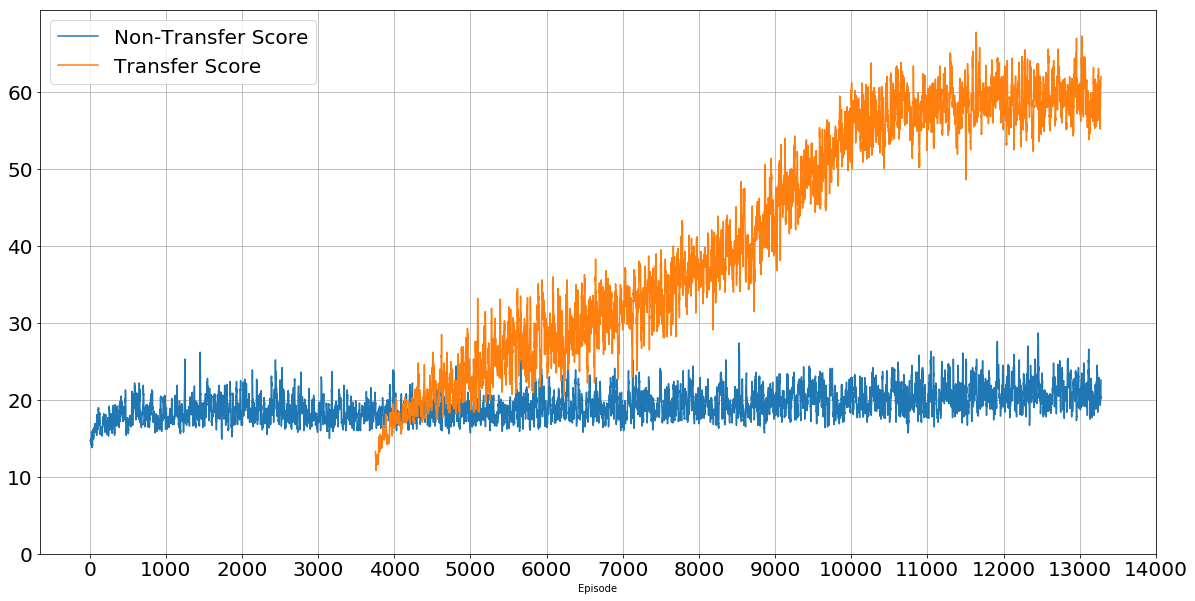
\includegraphics[width=0.97\textwidth]{cnn-transfer-move}
    \caption{Comparison of the rolling average achieved for the Transfer and
    Non-transfer learnt models.}%
    \label{fig:transfer_cnn_move}%
\end{figure}

The Deep Q agent was then tested on its ability to attack on multiple mini-games.
The agent was first trained on the FindAndDefeatZerglings mini-game. This map required
the agent to learn to search the map and kill the enemy units with little
strategy required. Next, the agent was tested on the DefeatRoaches and
DefeatZerglingsAndBanelings mini-games. The agent was able to show the correct
actions for the given state but with the limitation that the Deep Q agent is
unable to control individual units. This is a necessary skill to achieving a
higher score on these games as the agent needs to split the units and surround
the enemies. The overall performance was similar to the agent being trained on
each of the individual mini-games.

Finally, the convolutional network was also tested in its ability to move
between combat focused mini-games. However, like the Deep Q network, this did
not give any advantage in training time or performance as compared to the agent
trained solely on the DefeatZerglingsAndBanelings. In both cases, it is assumed
the reason there was no benefit is due to the different strategies used to
defeat each of the enemies. This meant a model trained to defeat Zerglings was
unable to defeat Banelings without a lot of training.

\section{Overall comparison}

Comparing the two networks, we can see that the Deep Q network can perform
well in mini-games that do not require a large action space, due to the complex
action sequences used by the Deep Q network. The Convolutional network, on the
other hand, can deal with games that have a large action space, but is
unable to easily formulate the more complex strategies needed for the later
mini-games.

This means the agents perform very differently in BuildMarines versus MoveToBeacon.
The Deep Q network can effectively use its more complex action space in
the BuildMarines game, but falls flat when it comes to the precise spatial
ability needed for the MoveToBeacon mini-game.

The Deep Q network also trains slower due to the single instance learning of the
value approximator. The agent needs to test different actions to find the
optimal value for a given state by playing the state multiple times. The Actor
Critic method used in the Convolutional network means that we can test different
instances of models being trained before combining the results. This allows many
instances of the game to be run at once, making training quicker. However, due
to the much larger action space and the lack of compound actions, the
Convolutional network does end up taking many more episodes to reach a strong
example.

Finally, it should be mentioned how the two networks compared to the published
scores. The MoveToBeacon game is the only game where the Convolutional network
matches the published DeepMind scores. After this, the scores are in a similar
range for the most part but do not match them exactly. As explained previously,
this is most likely due to the difference in hyperparameters and also in
training time. The network was able to beat the human player at the
DefeatRoaches mini-game however. The Deep Q network was able to beat the
DeepMind scores for the BuildMarines mini-game. However, both DeepMind and our
agents were drastically under either the human or professional players score.
That said, the Deep Q network was able to beat the Random Search policy, where
the Convolutional network did not.

\section{Network Information}

Figures~\ref{fig:dqn-scores-1} and~\ref{fig:dqn-scores-2} show the Deep Q score
during training. We can see the score dip as the epsilon value is reduced due to
the epsilon decay. The agent then learns the correct action to take in a given
state.

Figures~\ref{fig:cnn-filter1} and~\ref{fig:cnn-filter2} show the output of the
combined convolutional layer that is used to generate the spatial actions. The
images are given in greyscale, where the predicted best location is given in
white and gets darker the lower the probability. As can be seen, the
probability starts off very murky, with lots of noise, but after training
converges such that the only choice is moving to the target location. This can
be seen in the MoveToBeacon output as a single large point relating to the
current beacon position, and multiple small points for the CollectMineralShards
mini-game relating to the current shards.

\begin{figure}[h]
  \centering
  \begin{minipage}[b]{0.45\textwidth}
    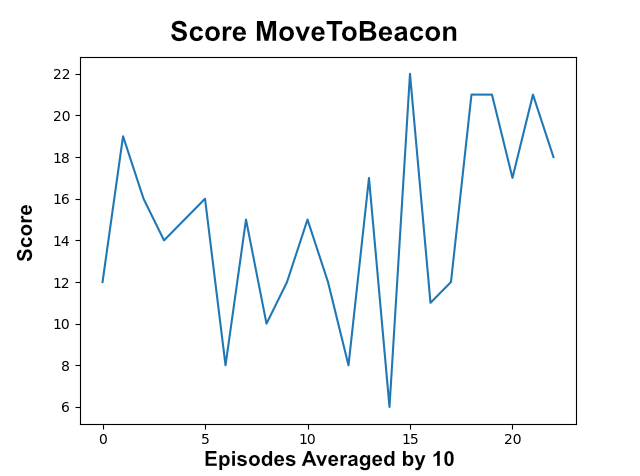
\includegraphics[width=\textwidth]{score_MoveToBeacon_train}
    \caption{Average of every 10 MoveToBeacon score during training}%
    \label{fig:dqn-scores-1}%
  \end{minipage}
  \hfill
  \begin{minipage}[b]{0.45\textwidth}
    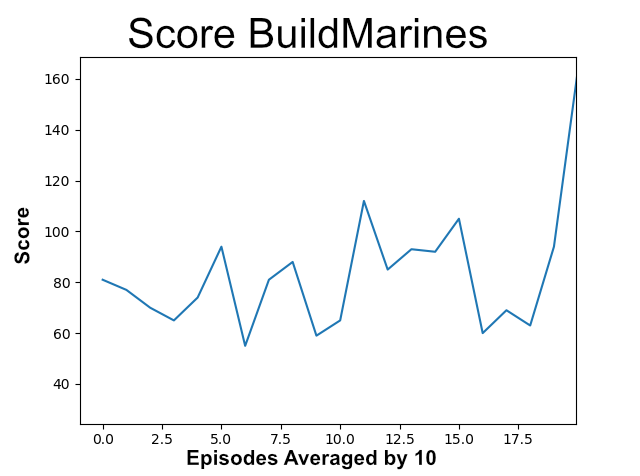
\includegraphics[width=\textwidth]{score_BuildMarines_train}
    \caption{Average score of BuildMarines runs during training, grouped over 10
    runs}%
    \label{fig:dqn-scores-2}
  \end{minipage}
\end{figure}

\begin{figure}[h]
    \centering
    \subfloat[Before training]{{
\includegraphics[width=0.45\textwidth]{Move_SmallTrain}}}%
    \subfloat[After training]{{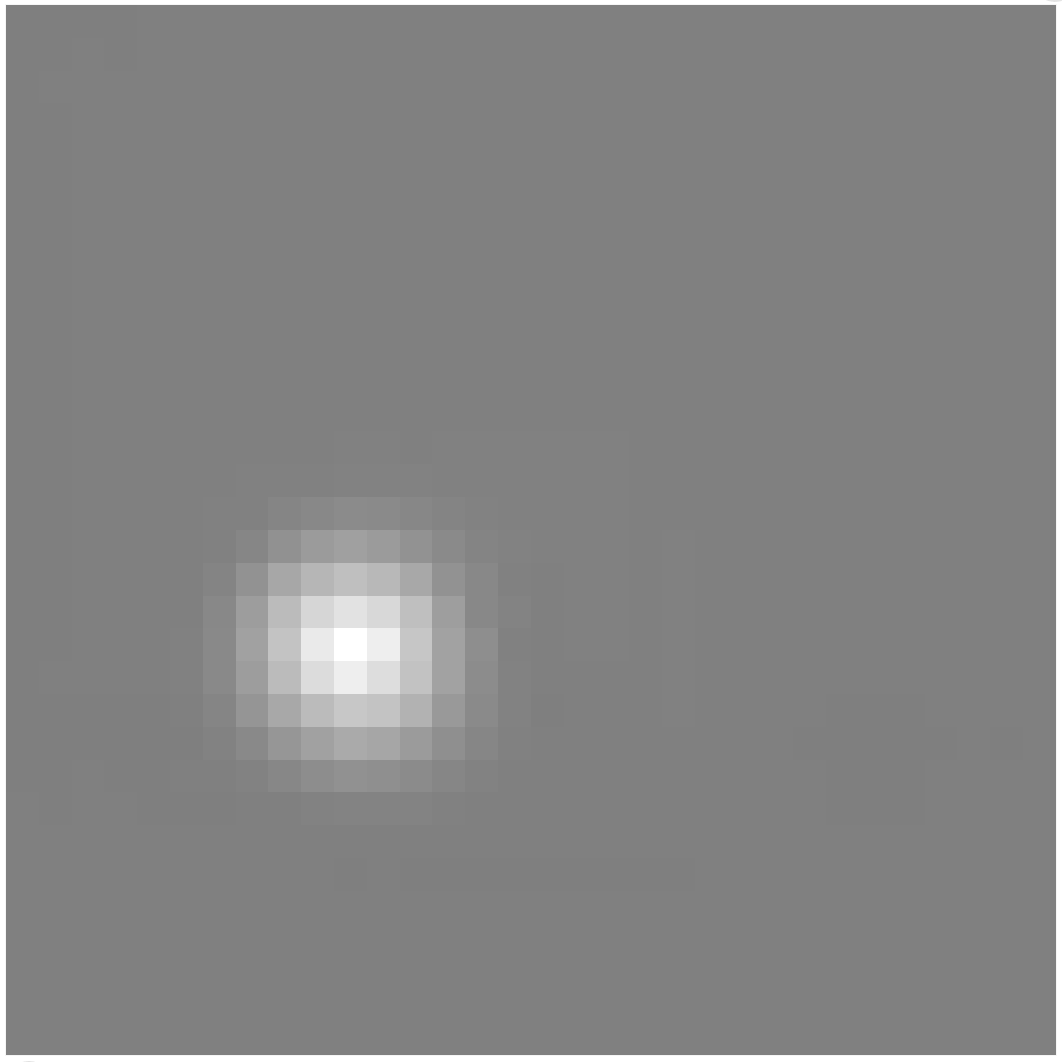
\includegraphics[width=0.45\textwidth]{Move_LotsOfTrain}}}%
    \caption{MoveToBeacon spatial action output before and after training.}%
    \label{fig:cnn-filter1}%
\end{figure}

\begin{figure}[h]
    \centering
    \subfloat[Before training]{{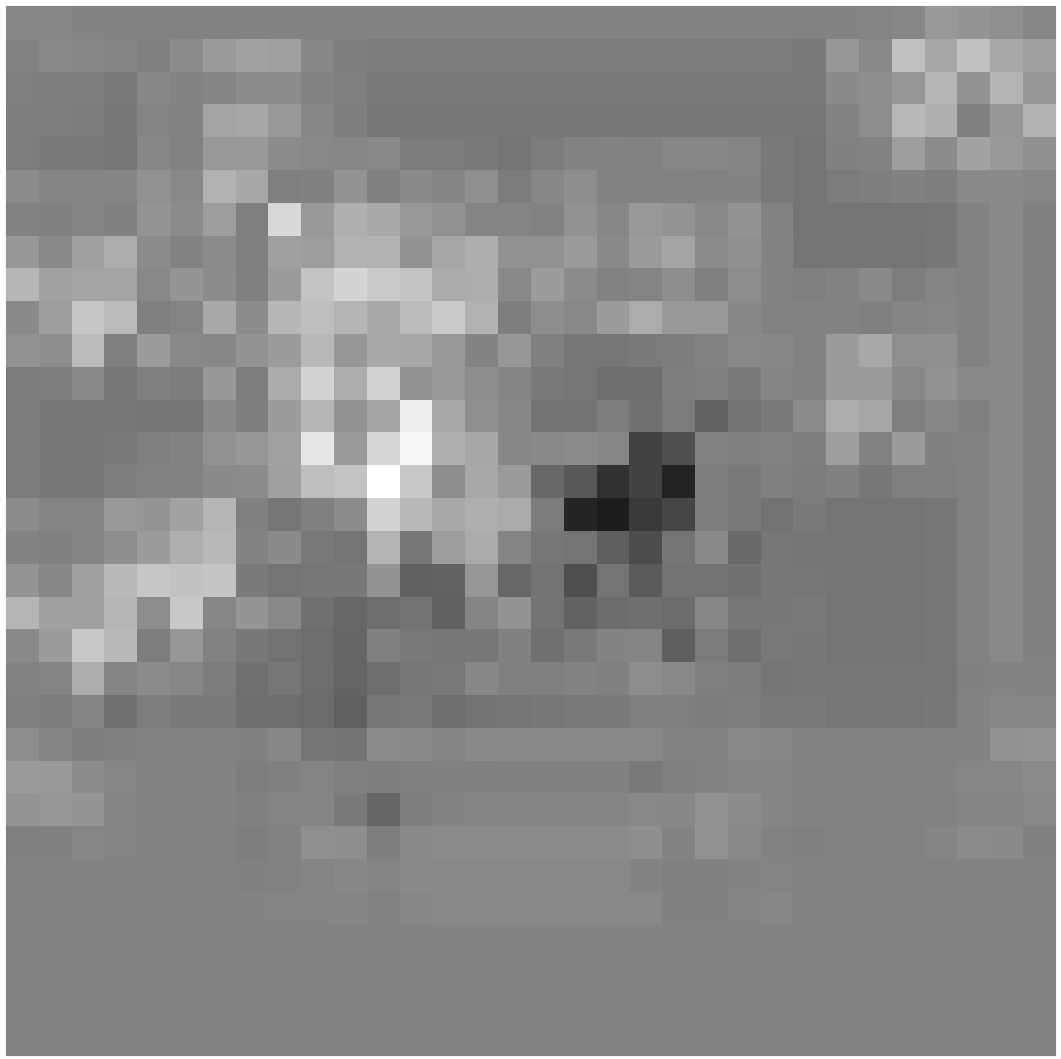
\includegraphics[width=0.45\textwidth]{Minerals_SmallTrain}}}%
    \subfloat[After training]{{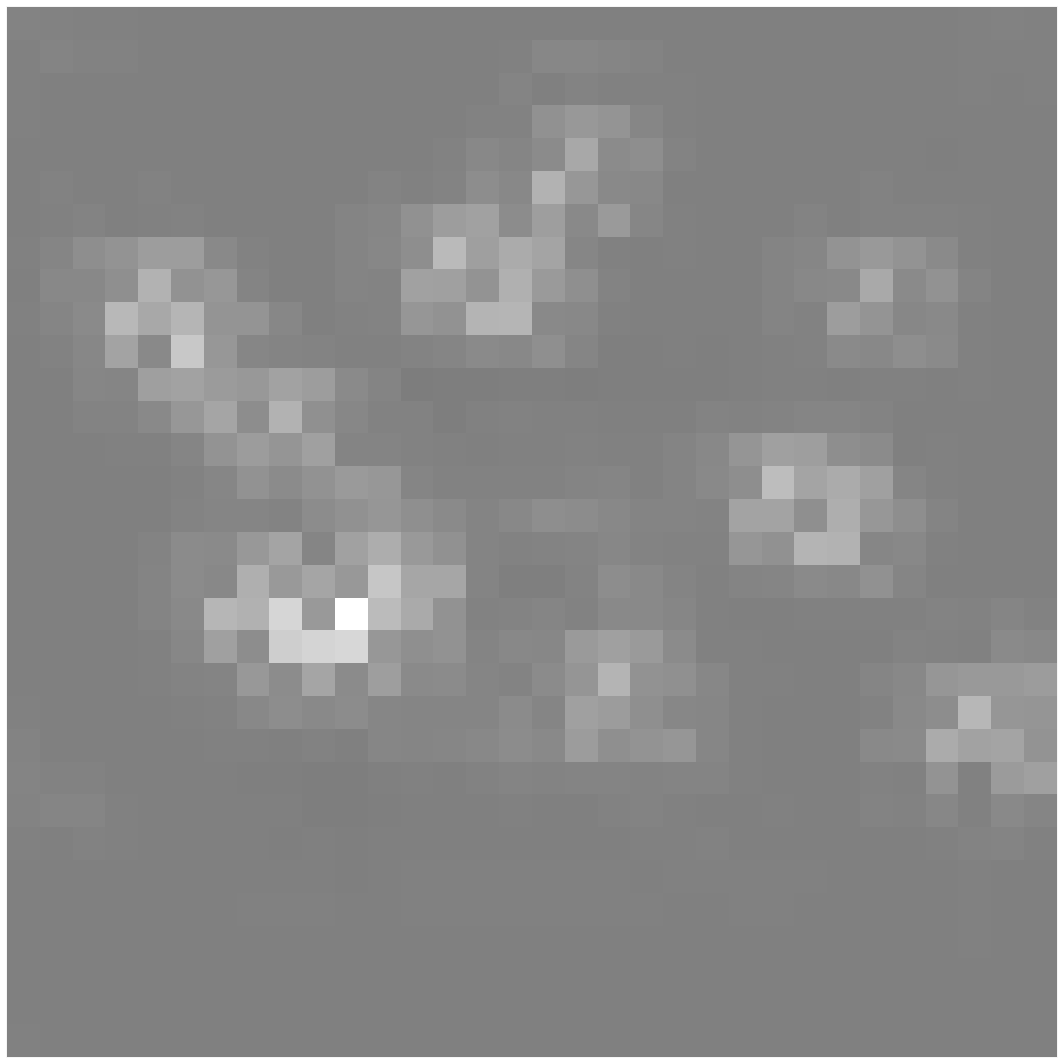
\includegraphics[width=0.45\textwidth]{Minerals_LotsOfTrain}}}%
    \caption{CollectMineralShards spatial action output before and after training.}%
    \label{fig:cnn-filter2}%
\end{figure}

\section{Conclusion}

Both networks were able to show a learning ability within each subsequent task.
They both were able to improve the base scores achieved at the beginning of
each training episode and showed they were learning towards improving their
scores. Additionally, the networks were able to learn certain behaviours from
different maps and apply the same abilities to some of the other maps.

The convolutional network required much more training time but was able to
outperform in any mini-game that required precise location-based actions such as
attacking and moving the units. In comparison, the Deep Q network had less time
but was able to perform better in maps that require a sequence of actions to
increase the score.

However, the networks were both limited by the size of the action and input
space. When both networks were increased to allow for more information, the
networks were unable to reasonably pick up the desired outcomes. Due to the
combinational possibilities of the input and output space, the networks would
need a much longer time of training to be able to learn and achieve a reasonable
score. Additionally, the bigger the action space, the harder it is for the agent
to find a smart set of actions to use.

Despite these issues, we can see that the agents were able to learn the
mini-games provided, and in some cases match or beat the performance of a human
player in those same games.

\chapter{Conclusion}%
\label{conclusion}

\section{Expansions of System}

As mentioned throughout the project, there are many things that could be
investigated, and other already included features that could be expanded.

To start, as spoken about briefly before, we could expand the Deep Q network,
such that it has a much richer action space. This would have two advantages.
Firstly, the agent should be able to learn more complex games and be more
accurate, as currently the action space is the main thing limiting the agents
abilities. This should make it score higher and as such, move closer to a more
intelligent and optimal solution. Secondly, this would have the advantage of
allowing the agent to behave more like a human. That is, despite the agents
compound actions giving it an advantage in the learning process, it is also
unrealistic as compared to a human player, who does not have the option of one
action that then performs many actions. Hopefully with a large enough action
space the agent would be able to learn these actions by itself.

Next, the convolutional network could be expanded. Firstly, this should include
the inclusion of non-spatial information such as resource and unit counts, such
that they can help influence decisions. This would bring it in-line with the
`FullyConv' specification that DeepMind speaks about in their paper. Similarly,
after this, the network could be expanded further to include a Long-term short
term memory component, which is the next network DeepMind specified. These two
modifications would allow the network to have more information, as well as
retain information on past decisions to help make the current decision.

As mentioned during the research, a network that uses a teacher/student mechanic
could be used, to see if it helps it learn the more complex mini-games, or also
if it helps time to train on the simpler games. This could be applied to both
networks, to provide similar comparisons as transfer and curriculum learning were
used for here.

Finally, something the networks would potentially also benefit from is using a
later version of the SC2LE, which has pixel level classifications, rather than
the broad feature maps that are available in the most recent version. This could
help the convolutional method most, but would also raise many issues. The
current network architecture performs very well using a very small number of
convolutional layers since the images it uses are feature maps with very
distinct features. If this was instead swapped to pixel level data, then the
network could potentially be able to become more accurate as it would have the
smaller models rather than the blobs produced by the feature maps, but the
network would also need to be expanded suitably to be able to process the images
rather than feature maps. This adds to the training difficulty of such a network
and would require better feature detection to begin identifying different
objects. This is due to objects being able to overlap in the game, since the
game is a perspective
projection and is angled to the viewer. Meaning that 2 units can partially

Any of the features mentioned here could provide interesting further work for
a project, with the chance of also increasing the performance of the networks
outlined here.

\section{Deliverables}

In Chapter~\ref{intro} a number of objectives and deliverables were defined, and
can now be assessed. The objectives the project set out to achieve are as
follows:

\begin{enumerate}
    \item The understanding and precise definition of the project space, that is
        what techniques will be used to tackle the problems, as well as metrics
        to measure the performance of a given prototype.
    \item A prototype (or multiple using various techniques) that exhibit
        intelligent behaviour in some behaviour in a given scenario for
        the game StarCraft II\@.
    \item Performance analysis of the given prototypes, such that their
        effectiveness can be measured and compared to other solutions, both of
        our design and as defined in other papers.
\end{enumerate}

And the deliverables outlined were:

\begin{enumerate}
    \item A Git repository containing the prototypes and any other associated
        code for getting the agents running.
    \item Associated learnt weights for each of the given agents, such that
        their performance can be easily tested without having to retrain
        the network.
    \item The evaluation of each of the given agents, alongside a full report
        detailing the rest of the project.
\end{enumerate}

Now at the conclusion of the project, these objectives can be reflected upon. Of
the three objectives outlined, all of them were met. This includes a full
chapter outlining both the current methods used for reinforcement learning in
games, as well as the theory behind the techniques. This was used as the basis
for the associated prototypes that were then made for the second objective. This
ended up being two main prototypes, with various tweaks applied to both to
optimise performance. The effectiveness and subjective intelligence of these
agents depends on the scenario at hand, but each are able to act intelligently
in given situations. Finally, to prove the intelligence of the agents beyond
simply subjectively watching them play, performance metrics were gathered from
the mini-games and Simple64 map, such that the performance could be more easily
compared. These scores were compared against published scores when possible, and
also subjectively analysed to ensure they were acting intelligently.

Similarly, the deliverables outlined were all met. All code throughout the
project was kept in a code repository to track changes that were made to the
agents over time, and also to allow easier collaboration between members. The
learnt weights are stored separately due to size and not being suitable to store
inside of version control. Finally, a full performance evaluation and report was
given containing all the research, implementation and evaluation that went into
the project, as well as methodologies for performing these steps where
appropriate.


\section{Conclusion}

In conclusion, this project achieved the aims that it set out to reach,
producing agents that were able to exhibit intelligent behaviour in the game
StarCraft II, and also experiment with the usage of transfer and curriculum
learning with them.

The project focused on the implementation and feasibility of 2 agent
architectures. The main focus was on the different aspects of running these 2
architectures with the usage of curriculum and transfer learning. We were able
to implement and design 2 networks that would play and learn from an in-game
environment. The most difficult aspect of the implementations was in the reward
engineering of a real-time game. This required the most time in development and
was never a complete aspect, as more possible functions could be created and
tested to improve the performance of the agents. However, since the agent needed
to transfer and learn from different maps, the reward needed to be generalised
so that the agent could use the same function on all the mini-games.

Using PySC2 and TensorFlow also introduced some difficulties with developing the
agents. Some of the runs gave internal errors from the TensorFlow API and the
usage of PySC2 required more research due to the poor documentation on the API's
implementation and feature system.

That said, despite the setbacks two agents were made that provide a useful
baseline for further work, as both a comparison target and as an example of how
a StarCraft II agent should look. This should allow further work to be performed
more easily, allowing research to happen faster.

Throughout the project, we could see that the networks required the minimal amount of complexity such that the agents can still perform well. Features needed to be especially selected so that the agent can benefit from the given information without making the network too large in its inputs. This difficulty can been throughout the architecture of the Deep Q network. Starcraft 2 is a real-time strategy game and is difficult for any form of machine learning. There were no turns and the agent needed to identify the optimal move every step of the game. However, we have shown that an agent can be taught to play the game. Better scores could be achieved with more complex networks but at the cost of performance and the amount of training time required. 

The networks have shown promising abilities to further advance and improve with more training time on a larger input and output space. Neural networks have a possible future in real-time games and, with the development of more computational power and better network structures, could in future iterations show real-time learning abilities to adapt to the opponent in the middle of a game.

%Adds References to the table of content
%all you bibtex entries go in the file called refs.bib
\addcontentsline{toc}{chapter}{References}
\printbibliography{}

%any appendices you have go in a file called appendix.
\begin{appendices}
\chapter{External Material}

\section{Code Repository}
The code used for this project may be found at
\url{https://github.com/CrossR/meng_project}. This does not include the
trained weights for Convolutional network due to a single model being close to
1GB in size. These can be provided upon request however.

\section{Used Materials}
As part of the project, we made use of the following resources:

\begin{itemize}
    \item StarCraft II --- \url{https://github.com/Blizzard/s2client-proto}
    \item The PySC2 API --- \url{https://github.com/deepmind/pysc2}
    \item TensorFlow --- \url{https://www.tensorflow.org/}
    \item Initial Q Learning Agent --- Used for initial Q Learning Agent ---
        \url{https://github.com/MorvanZhou/Reinforcement-learning-with-tensorflow}
    \item Convolutional Agent Flags --- Used for initial convolutional agent
        flags ---\url{https://github.com/xhujoy/pysc2-agents/blob/master/main.py}
    \item Convolutional Agent Initial Design --- Based on DeepMind's
        implementation, and modified from a recreation ---
        \url{https://github.com/pekaalto/sc2aibot}
\end{itemize}

\chapter{Ethical Issues Addressed}
The project aimed to create a specialised AI designed to solve an artificial
problem with no direct real-world applications.
No specific ethical concerns need to be addressed or were within the scope of the
project.

\end{appendices}

\end{document}
